\begin{savequote}[75mm] 
If I have seen further it is by standing on the shoulders of giants
\qauthor{Isaac Newton} 
\end{savequote}

\chapter{Introduction} \label{ch:introduction}

\newthought{Bioinformatics by it's very nature is multi--disciplinary}: biotechnology methods are used to capture data, mathematical and statistical models are necessary to make sense of it, and software/hardware is necessary to process all the information,  all of which should be seen from the viewpoint of existing biological knowledge.

Techniques and methods of uncovering the logic behind cellular processes are in constant development. The success of these methods is usually related to the ability to isolate a particular state/measurement of the organic material (e.g. level of expression of a single protein, number of mutations of a gene in a population, etc.). However,  cellular functions of a higher level and organism's processes can only be studied with a more holistic approach.

Integrating information from different experiments in the context of the current knowledge-base is one of the most recurrent duties that researchers have to accomplish. This task however takes on another dimension when the goal is to connect related data sets in a general way. For example, a researcher usually needs to connect the target gene of one experiment with the information about the protein in which it is known to be expressed.  However this becomes far more difficult if the aim is to automatically connect a whole dataset of genes and their protein products.

The challenges of integrating heterogeneous datasets range from technical (e.g. incompatibilities of the storage systems) to structural (e.g. two datasets can refer to the same entity using different identifiers), but overall the major challenge is to not lose the meaning of the connection e.g. linking proteins and genes, and knowing what their relationship is.

Integration of data usually refers to connecting data at a low level, by means of storing aggregated information from several sources or by saving links to where the source is. However it is also possible to integrate it at a higher level, where information is not saved and the aggregates are built and visualized on demand.

This project explores both the integration and visualisation of information in bioinformatics; the rest of this introduction presents both the state of the art and fundamental technologies in both fields. Chapter \ref{section:integration} presents the efforts made during this doctorate that contribute to the methods on how data are integrated in bioinformatics projects. Chapter \ref{section:visualisation} describes our inputs to the visualisation of data in bioinformatics, focusing in particular on a web tool for the visualisation of protein-protein interactions. The final chapter contains the conclusions of the project.

\section{Integration of information}
\subsection{State of the art}
The latest version of the Nucleic Acids Research NAR Database Issue added a further 58 databases to the online collection held by the journal, which then reached the number of 1552 databases \cite{FER2014}. This collection is far from including every single database, but it is  a good reflection of the number of available resources.
The approaches to integrate data from all these sources are themselves heterogenous, and are focused on different types of integration, from simply linking resources to development of complex structures of aggregated information. In \cite{GOB2008} the authors categorise the different techniques used to integrate data in bioinformatics into eight approaches, and then these categories were reorganised in \cite{ZHA2011b} into: data warehousing, federated databasing, service oriented integration, semantic integration and Wiki-based integration.

We now present some of the most representative projects that have attempted to integrate data and offer a solution for this requirement in the bioinformatics field, by using one or more of the aforementioned approaches. \footnote{We have decided to include the description of the Distributed Annotation System in a separate section of this document, because it is the base-technology of the developments shown in Chapter 2, and therefore it requires an extended description.}

\subsubsection{Data warehousing} \label{subsec:dwh}
It is centralised repository where the information from different sources is copied and processed to be kept  in a single place providing a single access point to their data. However the preprocessing of the data is usually a complex process and the posterior additions or editions might require a lot of work.

\paragraph{BioWarehouse}
BioWarehouse is an open source toolkit to create data warehouses using MySQL or Oracle \cite{LEE2006}. The motivation behind this project is to provide  a single access point that supports Standard Query Language SQL running in a high performance environment.
This projects follows the data warehousing approach to integrate data, however the authors argue that it can be used as a part of a federated system and therefore, it doesn't aim to replace existing distributed systems but rather to complement them.

The development efforts were focused on the creation of a relational data model that supports the information from several biological entities. Figure \ref{fig:biowarehouse} shows the main datatypes that are defined in the BioWarehouse scheme including: Taxon, BioSource, Nucleic Acid, Gene, Protein, Feature, Reaction, Chemical and Pathway. It was the objective of the creators that the model evolves to include other entities, but at the same time keeps the model as simple as possible.

The package that comprises BioWarehouse includes a set of loaders implemented in java and C++, that allows the automation of the process of loading data from several popular sources. 

An instance of BioWarehouse called Publichouse is available online \url{https://publichouse.ai.sri.com/phpmyadmin/} (last checked December 2014) and provides access to compiled data from: NCBI Taxonomy, Enzyme, MetaCyc Chemical Compound Ontology, MultiFun Gene Ontology, MetaCyc Pathway Ontology, BioCyc, Swiss-Prot and TrEMBL.

\begin{figure}  
\centering
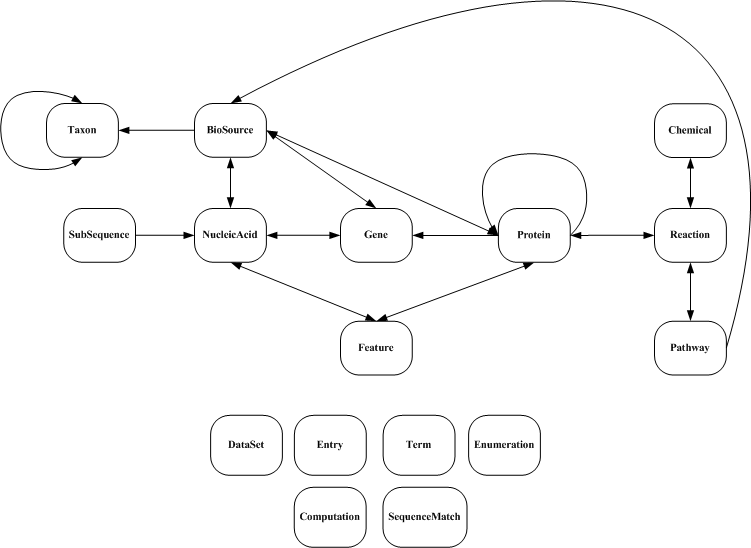
\includegraphics[width=5in]{figures/biowarehouse.png}
\caption[Original BioWarehouse schema.]{The main datatypes in the BioWarehouse schema, and the relationships between them.
\label{fig:biowarehouse}}
\end{figure}

The most recent contribution reported on their website is from August 2010 and includes the installation of the web based interface for mysql databases called myphpadmin. This highlights the lack of development that the project has had in the last 4 years. A similar situation has been observed in projects that follow the same warehousing strategy in bioinformatics. Most of them were published around the same period of time but have been inactive in recent years, or have broken links to the tool, for example, Atlas \cite{SHA2005} published in 2005, LCB\cite{AME2006} published in 2006 and M-Chips \cite{FEL2002} from 2002. From our research, the only active project on infrastructure of data warehousing for biological data is BioDWH, which is described below.

\paragraph{BioDWH}
The data warehouse for life science data integration known as BioDWH is a project developed at the Bielefeld University. BioDWH is a Java based project that developed an object-relational mapping using the library Hibernate to connect to the most common relational database management systems RDBMS (e.g. MySQL, Oracle, PostgreSQL) in order to create a centralised repository that integrates information from various biological databases \cite{TOP2008}.

BioDWH's main objective is to increase customisation of the data warehouse concept improving performance, scalability and having quality data up to date. As part of the project they have included some parsers to extract information from well-known available resources (e.g. UniProt, KEGG, OMIM, etc.). Figure ~\ref{fig:biodwh} presents the extensions to a general data warehouse design done in this project in order to define an architecture oriented to life sciences data.

\begin{figure}  
\centering
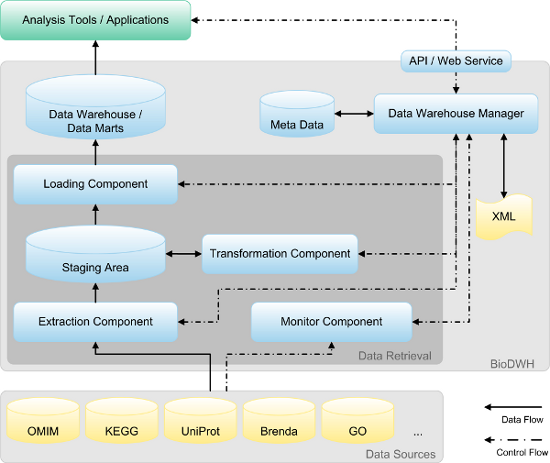
\includegraphics[width=4.5in]{figures/dwh_architecture.png}
\caption[BioDWH System Architecture.]{BioDWH System Architecture.
\label{fig:biodwh}}
\end{figure}

It is important to highlight the inclusion of a monitoring system that keeps track of the need for updates from the different sources. Instead of direct access to the RDBMS, BioDWH provides an API that can be queried remotely, and a Graphical User Interface that enables the configuration of the different components including monitors and parser along with the queuing and displaying of content.

Two projects have been reported in the literature that are using BioDWH: DAWIS-M.D. and VANESA. DAWIS-M.D. is oriented to metabolic data and integrates eleven different databases: BRENDA, EMBL, HPRD, KEGG, OMIM, SCOP, Transfac, Transpath, ENZYME, GO and UniProt \cite{HIP2010}. VANESA uses DAWIS-M.D. in order to access important information for the modelling of biological processes and systems as biological networks \cite{BRI2014}.

\paragraph{BioMart}
BioMart started by using the same principle as BioWarehouse, BioDWH and other projects of data warehousing in life science: ``\emph{to create one universal software system for biological data management and empower biologists with the ability to create complex, customised datasets}'' \cite{KAS2011}.

With this object in mind, BioMart has grown from an extension to the Ensembl website for data mining, to become an international effort for the integration of biological data. This has been achieved by first defining a general software infrastructure for further customisation, and then extending this architecture in order to support multi-database repositories as a data federation system, where all the entities use a predefined relational schema that is generic enough to support any kind of data.

\begin{figure}  
\centering
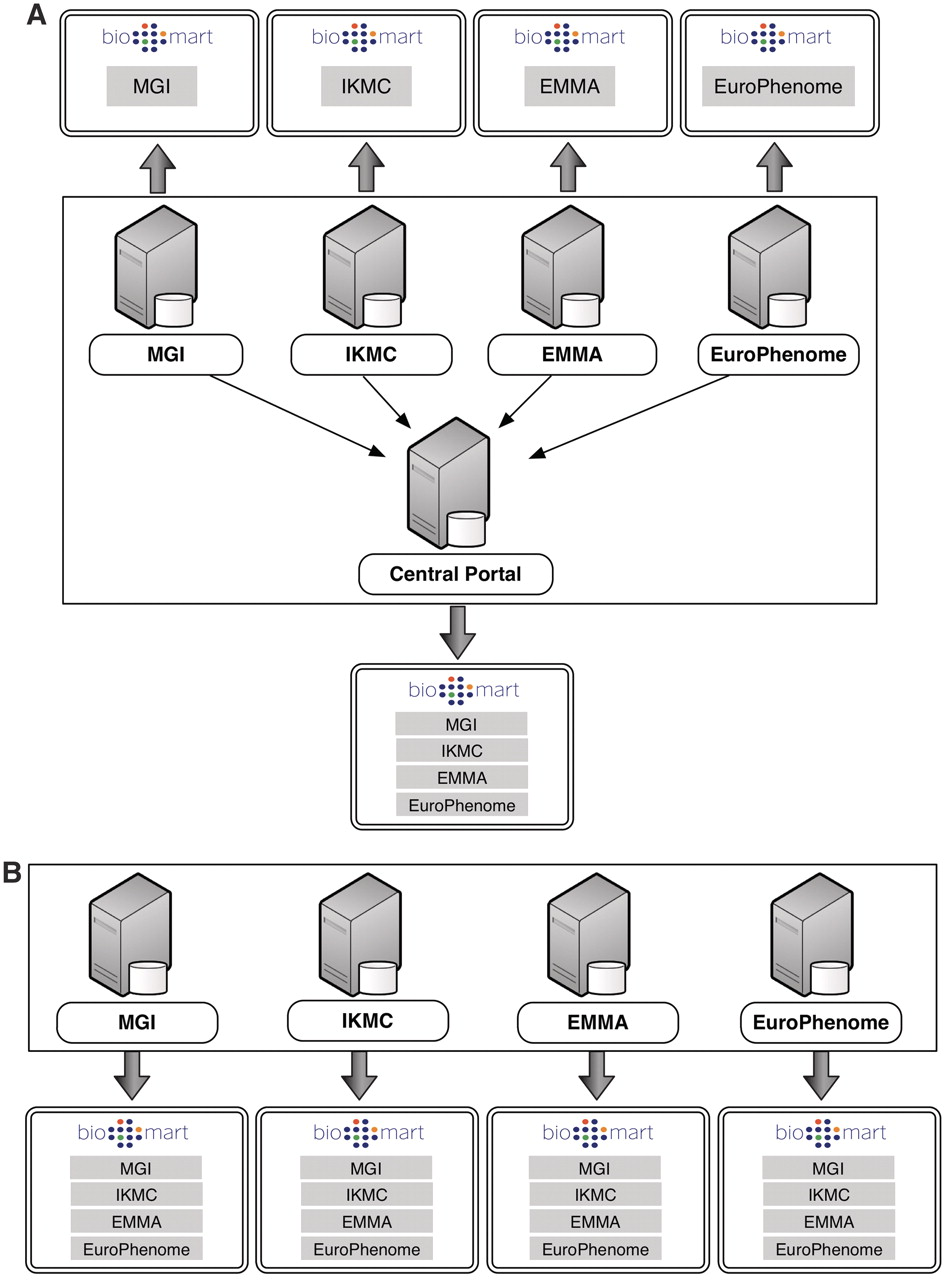
\includegraphics[width=5in]{figures/biomart.png}
\caption[Biomart Portal Architecture.]{Biomart Portal Architecture. The portal can be set either with a master/slave or with a peer-to-peer configuration.
\label{fig:biomart}}
\end{figure}

Given the inclusion of a multi-database paradigm, the BioMart team developed a server that provides access to a collection of sources called a BioMart Portal. Figure \ref{fig:biomart} shows the two possible configurations of the BioMart Portal. In configuration (a) each data source serves their own data and an independent server works as a central portal generating a unified view of the whole system. Alternatively, in configuration (b) all the data sources are treated as peers and they communicate with each other in order to be able to provide not only their own data, but also their peer's data.

BioMart includes a tool to automatically transform any 3rd form normalised database schema into the reverse-star scheme type used by this system. Once the dataset has been transformed, BioMart provides different view ports to it: Web-based Graphic Interface, Restful services and API connectors using Java \cite{KAS2011}.


\subsubsection{Federated databasing} 
This approach requires the agreement of multiple sources to follow a similar structure in order to allow a standard query over several instances. By dealing with smaller datasets than the data warehousing approach, the complexity of post-processing is simplified, however it requires that the providers deal with the extra work of maintaining their data as the federated database agreement establishes.

\paragraph{The HUPO Proteomics Standards Initiative}
The Proteomics Standards Initiative (PSI) is a collaborative initiative run by volunteers and coordinated as a work group of the HUman Proteome Organisation (HUPO), whose object is to define standards  to enable capture, comparison, exchange and verification of proteomics data. \cite{HER2006}. PSI is the result of a common effort from the interested parties in the proteomics domain.

This effort can be categorised into three major infrastructure elements: (1) A specification of the Minimum Information About a Proteomics Experiment (MIAPE), (2) data exchange formats that are compliant with MIAPE, and (3) the use of controlled vocabularies (CV) in order to ensure consistency on the data content. In this way the proposed standard can be stable while its content can evolve by updating the CV.

These recommendations are not intended to specify the methods and procedures for proteomics experiments, and should be seen as reporting guidelines.

This initiative has been growing for the last 10 years, and now its standards are widely adopted in the proteomics community. The proposed specifications cover different branches of the field, for instance the PSI-MI formats were defined to deal with Molecular interaction data, PSI-MS works on standards for mass spectrometry data and PSI-MOD focuses on protein modifications.

However even if all the parts follow the recommendations, a strategy to integrate this data is required. It is for this reason that the PSI common query interface (PSICQUIC) was created: a community standard that enables programmatic access to molecular-interaction data resources \cite{ARA2011}. This proposal includes a query language (MIQL) and an architecture to execute a query on distributed sources.
\label{subsec:psicquic}
Figure \ref{fig:psicquic} shows the architecture of PSICQUIC. The idea is that several samples from an organism can be processed by different experiments, and their findings can be published in independent articles, which consequently can be stored in more than one interaction database. PSICQUIC proposes that the providers include an extra layer to access this information, which can be queried using MIQL and with responses following the PSI-MI formats. In this way a client can use a single query over multiple resources and create a unified image.

\begin{figure}  
\centering
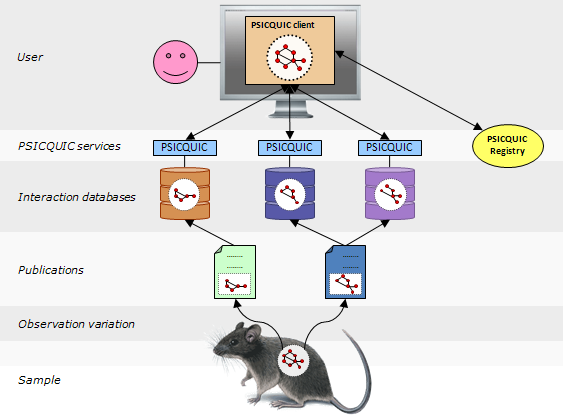
\includegraphics[width=4.5in]{figures/psicquic.png}
\caption[PSICQUIC Architecture.]{PSICQUIC Architecture.
\label{fig:psicquic}}
\end{figure}

The PSI group recognises the importance of providing software tools to promote the adoption of the proposed standards. The most recent implementation of the PSICQUIC web service was released when version 1.3 of the PSICQUIC specification was made public in 2013 \cite{DEL2013}. The providers of molecular interaction data are now asked to implement a number of methods in order to support both SOAP and REST web services. 

The web service methods will generally accept a MIQL query as input and generate an output in either PSI-XML or PSI-MITAB in its most recent versions. This implementation is based on the Apache Solr indexing software (\url{http://lucene.apache.org/solr/}), and is reflected in the constitution of MIQL, which is an extension of the Lucene query language used in Solr. This implementation is freely available for any provider who wishes to share their data to the PSI community.

Besides the server, PSICQUIC also provides client libraries to facilitate access to the information from three different programming languages: Java, Perl and Python. There are ready to use clients, for example the PSICQUIC View accessible from \url{http://www.ebi.ac.uk/Tools/webservices/psicquic/view/main.xhtml} or plugins for Cytoscape and the R Bioconductor package.

The last component of the PSICQUIC architecture is the registry, in which information about the available providers is stored as tags. This metadata can be used to query the registry as a RESTful service in order to facilitate the discovery of molecular-interaction data providers \cite{DEL2013}.


\subsubsection{Service oriented integration} 
The principle of service oriented integration is to have atomic components that offer a basic service. These services can then be connected in order to orchestrate the execution of a bigger task. Services can be data providers but can also be programs that execute specific functions.

The definition of a protocol for requests and responses to obtain data or execute services is the key to facilitate the connectivity between the software components. The two standards most widely used are SOAP (Simple Object Access Protocol) services and REST (REpresentational State Transfer) services, where the latter is gaining momentum because of its simplicity. However service oriented integration also requires a large commitment from providers in creating and maintaining the services, and also increasing and maintaining the specifications for the different domains. A comparison between SOAP and REST web services can be found in \cite{PAU2008}.

Alternatively, the services can run on a local installation, which does not follow the principle of a unique remote resource executing a service to multiple consumers. Nonetheless, this option has been widely used in bioinformatics environments in order to have more control over the data and services offered.

\paragraph{Sequence Retrieval System}

The Sequence Retrieval System, better known in bioinformatics as SRS, was probably the most successful project before the introduction of Next Generation Sequencing (NGS) technologies, originally aimed at facilitating access to biological sequences databases \cite{ETZ1996}. It grew to become an integration system of both data retrieval and applications for data analysis.

SRS was developed following an object-oriented design with the strategy of taking advantage of raw text files, that were the \emph{de-facto} standard on molecular biology analysis. By dealing only with text files, SRS was getting faster retrieval speeds and saving storage space, mainly because data was neither stored nor parsed, only indexed \cite{ZDO2002}.

The  indexes obtained were linked via meta-data, offering the user access to the original source plus links to any conceptually related database. This was then presented in a web-based interface. The automatically created interface for different sources and applications can be complicated for beginners, however SRS provides ways to create customised interfaces.

Probably the most important instance of SRS was the one installed at the European Bioinformatics Institute (EBI), which was used to provide access to the major databases produced and maintained at the EBI. However by December 2013 the service was decommissioned as the service was considered redundant with the efforts to maintain multiple web services. Currently SRS technology is the property of Instem\textsuperscript{TM} and a list of available servers can be found at \url{http://bioblog.instem.com/download/srs-parser-and-software-downloads/public-srs-installations/}.

\paragraph{Taverna}
Taverna was originally conceived of as a tool for non expert programmers to design, execute and share workflows of web services \cite{HUL2006}. Bioinformatics web services can be a way of providing the available data in a data source (e.g. the PSI services), but traditionally, web services are seen as a remote software component that receives some input data, processes it and generates output data. The main advantage of using web services  is that most of the processing load is delegated to the service provider, allowing small groups to run high throughput analysis in remote but powerful machines.

Taverna is a tool that allows the user to create ``recipes'' of combined web services or pre-composed workflows to execute a higher level computational experiment. The Taverna workbench is a graphical interface that allows the design of workflow, that can be executed either on the same workbench or in independent runner tools such as the Taverna command-line application, the Taverna server or the Taverna lite installation.

By 2013 the Taverna project was reported to have access to over 8000 service operations \cite{WOL2013}. With such a large number of resources, there is a necessity to make them searchable. This is the goal of the BioCatalogue: a registry for web services where both REST and SOAP services can be discovered using their metadata. Taverna supports searching on the BioCatalogue and inclusion of a chosen web service through its workbench tool.

It is often necessary to do intermediate processing to be able to connect two services, where for example one produces the data that is required for the second but in a different format. Taverna provides a set of what they call ``shim'' services to cater for this need. Other types of services that are supported by Taverna are local, grid and cloud services, access to BioMart, R-Scripts and distributed command-line scripts.

The number of ready-to-use workflows have grown in recent years, which is ideal for researchers that need a starting point for their experiments. However this number is so large that finding the right pipeline for an analysis is not an easy task. For this reason MyExperiment was developed, it not only supports Taverna workflows but also other systems such as Galaxy (discussed below). To run a workflow found in the MyExperiment repository in Taverna is as easy as copying the URL into the workbench importer, adjusting the parameters and pressing ``run'' \cite{WOL2013}.

\paragraph{Galaxy}
Starting as a project to integrate genomic sequences, their alignments and functional annotations, Galaxy has evolved rapidly in less than 10 years to the point of offering a complete web-based framework that aims to enable reproducibility, accessibility and transparency for computational biology experiments \cite{GIA2005, GOE2010}.

First versions of Galaxy were written in a combination of C for the core components and Perl for the user interface, promising the possibility of adding new tools thanks to its architecture. Nowadays the project has been rewritten in Python and follows an open source strategy with over a hundred commits per month on its public repository (\url{https://bitbucket.org/galaxy/galaxy-central/overview}), and the extensibility promise has been fulfilled to the point of asserting that Galaxy supports any tool that can be run in the command line.

This feature marks the greatest difference between Galaxy and Taverna, because the latter has web services as its basic workflow unit while Galaxy is used to compose workflows using command-line tools.

Galaxy's main goal is to provide a tool where experiments can be reproduced easily and reliably; and Galaxy's authors consider that because it is in the nature of web services to be hosted by remote and probably unknown service providers, the reliability is compromised, and therefore web services are not natively included in Galaxy.

Despite the fact that the origin of Galaxy did not explicitly include the execution of workflows as its core functionality, Galaxy's detailed history of task executions has evolved and currently it offers all the advantages of a modern workflow execution suite.

The addition of metadata to both workflows and tools, and its publication by the means of Galaxy Pages makes the project easier to share. A well annotated workflow can be understood better when its documentation goes beyond the sequence of tools that have been connected, and includes the biological meaning of such executions.

There is an instance of Galaxy publicly hosted at \url{https://usegalaxy.org/} where a subset of features can be explored by anonymous users and the rest of the functionalities become available after free registration. This public tool includes hundreds of tools for getting data, processing it and visualizing it. If however, a project has particular requirements such as including non-public tools, Galaxy can be installed as a local server and the tools can be added to that instance \cite{GIA2005, GOE2010}.


\subsubsection{Semantic integration} 
The main methodology under semantic integration is to structure the data using semantic web standards (e.g. RDF, OWL) in order to make it ``machine-readable'' and be able to deduce meaningful associations. The conversion of the data into RDF files might not be a trivial endeavour, and it has similar problems to the ones mentioned above because it usually implies maintaining copies of the information in a separate format. 

\paragraph{BioMOBY}
BioMoby is one of the attempts to bring the promises of the semantic web into bioinformatics, proposing an architecture for the discovery and distribution of data though web services using multiple proposed standards of the World Wide Web Consortium (W3C) such as the Simple Object Access Protocol (SOAP). Its main goal is to provide access to biological data and services with a common format among the different sources \cite{WIL2002}.

The strategy of BioMoby is to define a minimalistic entity to describe the data in such a way that different types of data can use the same schema.
This structure has been called the MOBY object, and is composed of three values: the MOBY object type (e,g. Sequence), a namespace identifier (e.g. Genbank/AC) and an accession number (e.g. AY070397.1). MOBy object types are defined using XML Schemas (XSD) reflecting a hierarchical relationship between them.

An important component of the BioMoby ecosystem is MOBY Central: a server that contains information not only about available services, but also their association with MOBY objects for input and output. With this information a MOBY client can suggest paths to follow depending on the current type of your data. Moreover, the intrinsic semantics of this approach is the ideal environment in which to create cohesive workflows.

\begin{figure}  
\centering
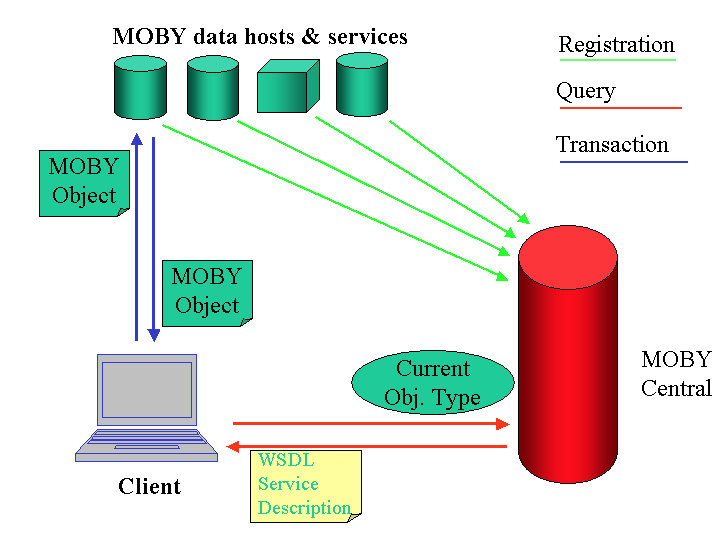
\includegraphics[width=4in]{figures/MOBY_Overview.png}
\caption[BioMoby Overview.]{BioMoby Overview.
\label{fig:biomoby}}
\end{figure}

Figure \ref{fig:biomoby} shows the adaptation done by BioMOBY to the classic web services architecture: once all services have registered with MOBY central, a client can query it to find out which services can be used with the current MOBY Object. Besides the discovery feature, the central repository has the capability of generating a Web Service Description Language (WSDL) document that can be used with the corresponding service, where both input and output are MOBY Objects.

A more recent iteration of the development of MOBY was described in \cite{VAN2009}: Moby-2. The objectives of the project have been extended and its focus on semantic web technologies is stronger: MOBY Central will take the form of a Resource Description Framework (RDF) triple store and will support the functionalities of a SPARQL endpoint. These changes were done with the objective of allowing semantic queries over multiple sources. The project was reported in \cite{VAN2009} as a prototype, but promised to contribute towards a distributed, machine-readable semantic web of life science data.

\paragraph{Bio2RDF}
A simplified view of the Semantic Web can be defined as a network where the nodes represent any entity that can receive a name and the edges correspond to the characteristics used to describe the relationships between the nodes. The RDF format is an XML-based language that describes this relationships as a set called a ``triple'' that contains subject, predicate and object.

Bio2RDF uses RDF documents to be able to create a knowledge base that takes advantage of existing developments on the semantic web to build a mashup of data in the bioinformatics domain.  \cite{BEL2008}.

One of the main objectives of Bio2RDF is to extract information from the most important bioinformatic databases, transform its content into RDF, and load it into a triple-store. It is within a triple-store that discovery of new knowledge occurs through recombination analysis of the loaded data. In this sense, Bio2RDF follows the approach of a data warehouse of semantic data.

As part of the project, a set of software tools that convert different datasets into RDF called ``Rdfizers'' were created. There is one rdfizer for each source, however they can be grouped in three types depending on the origin of the data: XML to RDF, SQL to RDF, and text file to RDF. For large scale resources such as UniProt or PubMed where programmatic access to the data is provided, the rdfizer works on-demand, which means that it only stores some of the data for cache purposes and the RDF files are created on the fly. Any other source gets copied into the centralised repository in order to offer quick responses.

The Bio2RDF approach can be summarised in three steps: (1) build a list of namespaces for data providers, (2) analyse a data source to represent it in an RDF model and (3) develop rdfizer to convert the information. The resulting dataset is sorted in the triple-store in order to connect it all together.

Bio2RDF used an extended version of Sesame as the triple-store and on its 2nd release was changed to Virtuoso in order to offer better support to SPARQL, which is the most widely used query language for semantic web data. Bio2RDF makes use of other tools such as Protégé: an ontology editor, the Piggy Bank: a semantic browser for Firefox and Welkin: a RDF graph visualizer; all of which are well known projects in the semantic web community \cite{BEL2008}.

\paragraph{SADI}
The Semantic Automated Discovery and Integration (SADI) project has its roots in the lessons learned from BioMoby, particularly  Moby-2. However, unlike BioMoby, SADI is not a data typing system. The goals of SADI are centred on the proposal of patterns and best practices of how to use web services connected through semantic web technologies to enable the creation of interoperable and integrative bioinformatics software. \cite{WIL2011}.

The biggest change introduced by SADI in respect to SOAP web services is to replace the defined languages for communication between the web services parts (e.g. WSDL, XML Schema,UDDI) with structured versions of semantic web languages: RDF and OWL. The authors go as far as to say that XML Schema is the problem causing the failure of most previous interoperability architectures.

A description of an interaction with a SADI service is as follows: A client requests the service description via HTTP GET, and the server responds with a document containing references to OWL classes describing input and output datatypes for the service. The client uses data formatted in RDF that follows the received description to submit an HTTP POST request, which is captured by the server, which in turn uses it to execute the service and generate a response in RDF format.

The adoption of HTTP methods for communication follows the positive reception of ``RESTful'' Architectures. SADI does not claim to follow a RESTful architecture, but it sees the potential of it and uses some of its principles. This is partially a response to the general dislike of the SOAP architecture within the bioinformatics community.

The use of a good ontology to connect services is seen in SADI as the key component to meaningful interoperability, where the interaction between servers is guided by biological knowledge and not only by technicalities such as format and availability \cite{WIL2011}.

As part of the project, software components have been developed in order to facilitate the adoption of the recommendations including plugins for Taverna and Protegé, and a  prototype of all the components (i.e. Servers and clients) is available at \url{http://biordf.net/cardioSHARE/}.


\paragraph{BioPAX}
The Biological PAthway eXchange (BioPAX ) is a community driven effort to develop a standard language to facilitate knowledge representation of biological pathways at molecular and cellular level in order to enable the systematic collection, distribution and integration of pathway data from heterogeneous sources \cite{DEM2010}.

BioPAX also takes input from the semantic web community. In this case OWL is used to define an ontology to describe pathway information, which can be used to interconnect the multiple resources in this domain. BioPax has, among others, been used to describe (1) metabolic pathways, following the abstraction: ``enzyme, substrate, product''; (2) signalling pathways for biochemical reactions, binding, and catalysis events; (3) gene regulatory networks involving transcription and translation events and its control; (4) protein-protein interactions and protein-DNA interactions; and (5) genetic interactions i.e. when the phenotype of perturbing two genes is different from the expected known phenotype of the perturbation of each isolated gene.

The BioPAX ontology is the result of ongoing periodical workshops that involve the different stakeholders in the biological pathways field. Incremental versions of the agreement, also called levels, have been developed with the concept that newer levels can replace older ones. Currently the highest  is level 3.

A tool set called Paxtools has been developed as part of the project. The main features of this software include an implementation of the specification as a software model, the support of OWL properties, a syntactic validator, transformation scripts between levels, import and export to other formats. Thanks to these features, Paxtools can and has been used as the framework to develop other tools \cite{DEM2010}.

\subsubsection{Wiki-based integration} 
It is a cooperative effort where the community inputs information in an open and unstructured way, which can reach a highly reliable status as has been shown in the case of wikipedia. It is however completely dependent on the adoption of the community, and also given the unstructured nature of the data, is hard to manipulate for automatic analysis.

\paragraph{WikiPathways}
Following the success of wikipedia, where any user can contribute to an article and the tasks of editing and curation are community based; WikiPathways has been developed with the objective of providing an open platform to deposit, share and curate biological knowledge in the form of pathway diagrams \cite{KEL2012}.

Biological pathways are representations of the compiled knowledge of biological units and their relationships. Pathways are vital to understanding genes and proteins in terms of larger systems and processes of any organism. The challenges of gathering knowledge about biological pathways are particularly hard: (1) pathway information is not measurable and can't be obtained from a single experiment, (2) many different representations and methods have already been used, and (3)  representations are usually saved as static images, which are far from ideal for computation and integration \cite{PIC2008}.

Looking to tackle these challenges and inspired by how science has been gaining a more open approach by means of open journals, public databases, data exchanges formats, ontologies and free software; WikiPathways provides a web based framework where the community can not only take information but also give back.

In WikiPathways, each pathway has a dedicated page that summarises the existing information around the specific biological mechanism including its diagram, description, links, related genes and proteins, and relevant literature references. The pathway is displayed using an interactive viewer that supports navigation and live highlighting. Registered users can also use the viewer to improve a pathway, and all the information can be exported in suitable formats such as the BioPAX standard.

A subset of the functions of the web-site can be programatically accessed via web services.

The metadata associated with the pathway serves the purpose of making it searchable, but most importantly makes it easy to integrate with other resources because it follows an ontology that as a side effect can be used to organise the created pathways in a hierarchical fashion.

Nonetheless it is clear to the authors that the tools and developments only assist in the community building process and its in the growth of the community itself that the future of WikiProteins is held \cite{KEL2012}.

\paragraph{WikiGenes}
In contrast to what its name suggests, WIkiGenes is not exclusively about genes; its scope goes beyond genes and aims to construct a knowledge base of biological information including chemical compounds, proteins, organisms, pathologies and of course genes. 

Similarly to WikiPathways, WikiGenes applies a strategy based on the wiki model, however in \cite{HOF2008} the author argues that given that the wiki model was not created taking into account the demands of the science ecosystem, it requires significant technical innovation. In particular, current wiki alternatives do not consider the current scientific publications paradigm, and the relevance of authorship. 

The advantages of having a continuously updated article on each topic are obvious, however the effort from contributing scientists to reach this goal is quite considerable and the personal benefits of such efforts are not very clear. Traditional scientific publications recognise the efforts of a contributor by clearly stating its authorship, which in today's academic world might get reflected in employment, grants and ultimately in the privilege of being a scientist.

WikiGenes proposes a system where every word of a document can be linked to its author in order to provide him/her with his/her due recognition. Such a document is reviewed by its readers as in the wiki model, however WikiGenes includes a reputation system that can be used to solve disagreements between authors and avoid vandalism.

More than a hundred thousand generated articles on several biomedical concepts have been included in WikiGenes. It is clear that the quality of these articles is not the best, but it serves as a starting point for interested authors \cite{HOF2008}.


\subsection{The Distributed Annotation System}
\label{ssec:DAS}
%\footnote{Most of the text in this section was originally included in the lead author's MSc dissertation\cite{SAL2010} and edited here to update it where necessary.}
The Distributed Annotation System (DAS) \cite{DOW2001} makes use of a widely-adopted standard communication protocol. It is motivated by the idea of maintaining a federated system; a logical association of independent sources distributed over multiple sites, which provide a single, integrated, coherent view of all resources in the federation. This architecture makes several distinct physical data sources appear as one logical data source to end-users. 

\begin{figure}  
\centering
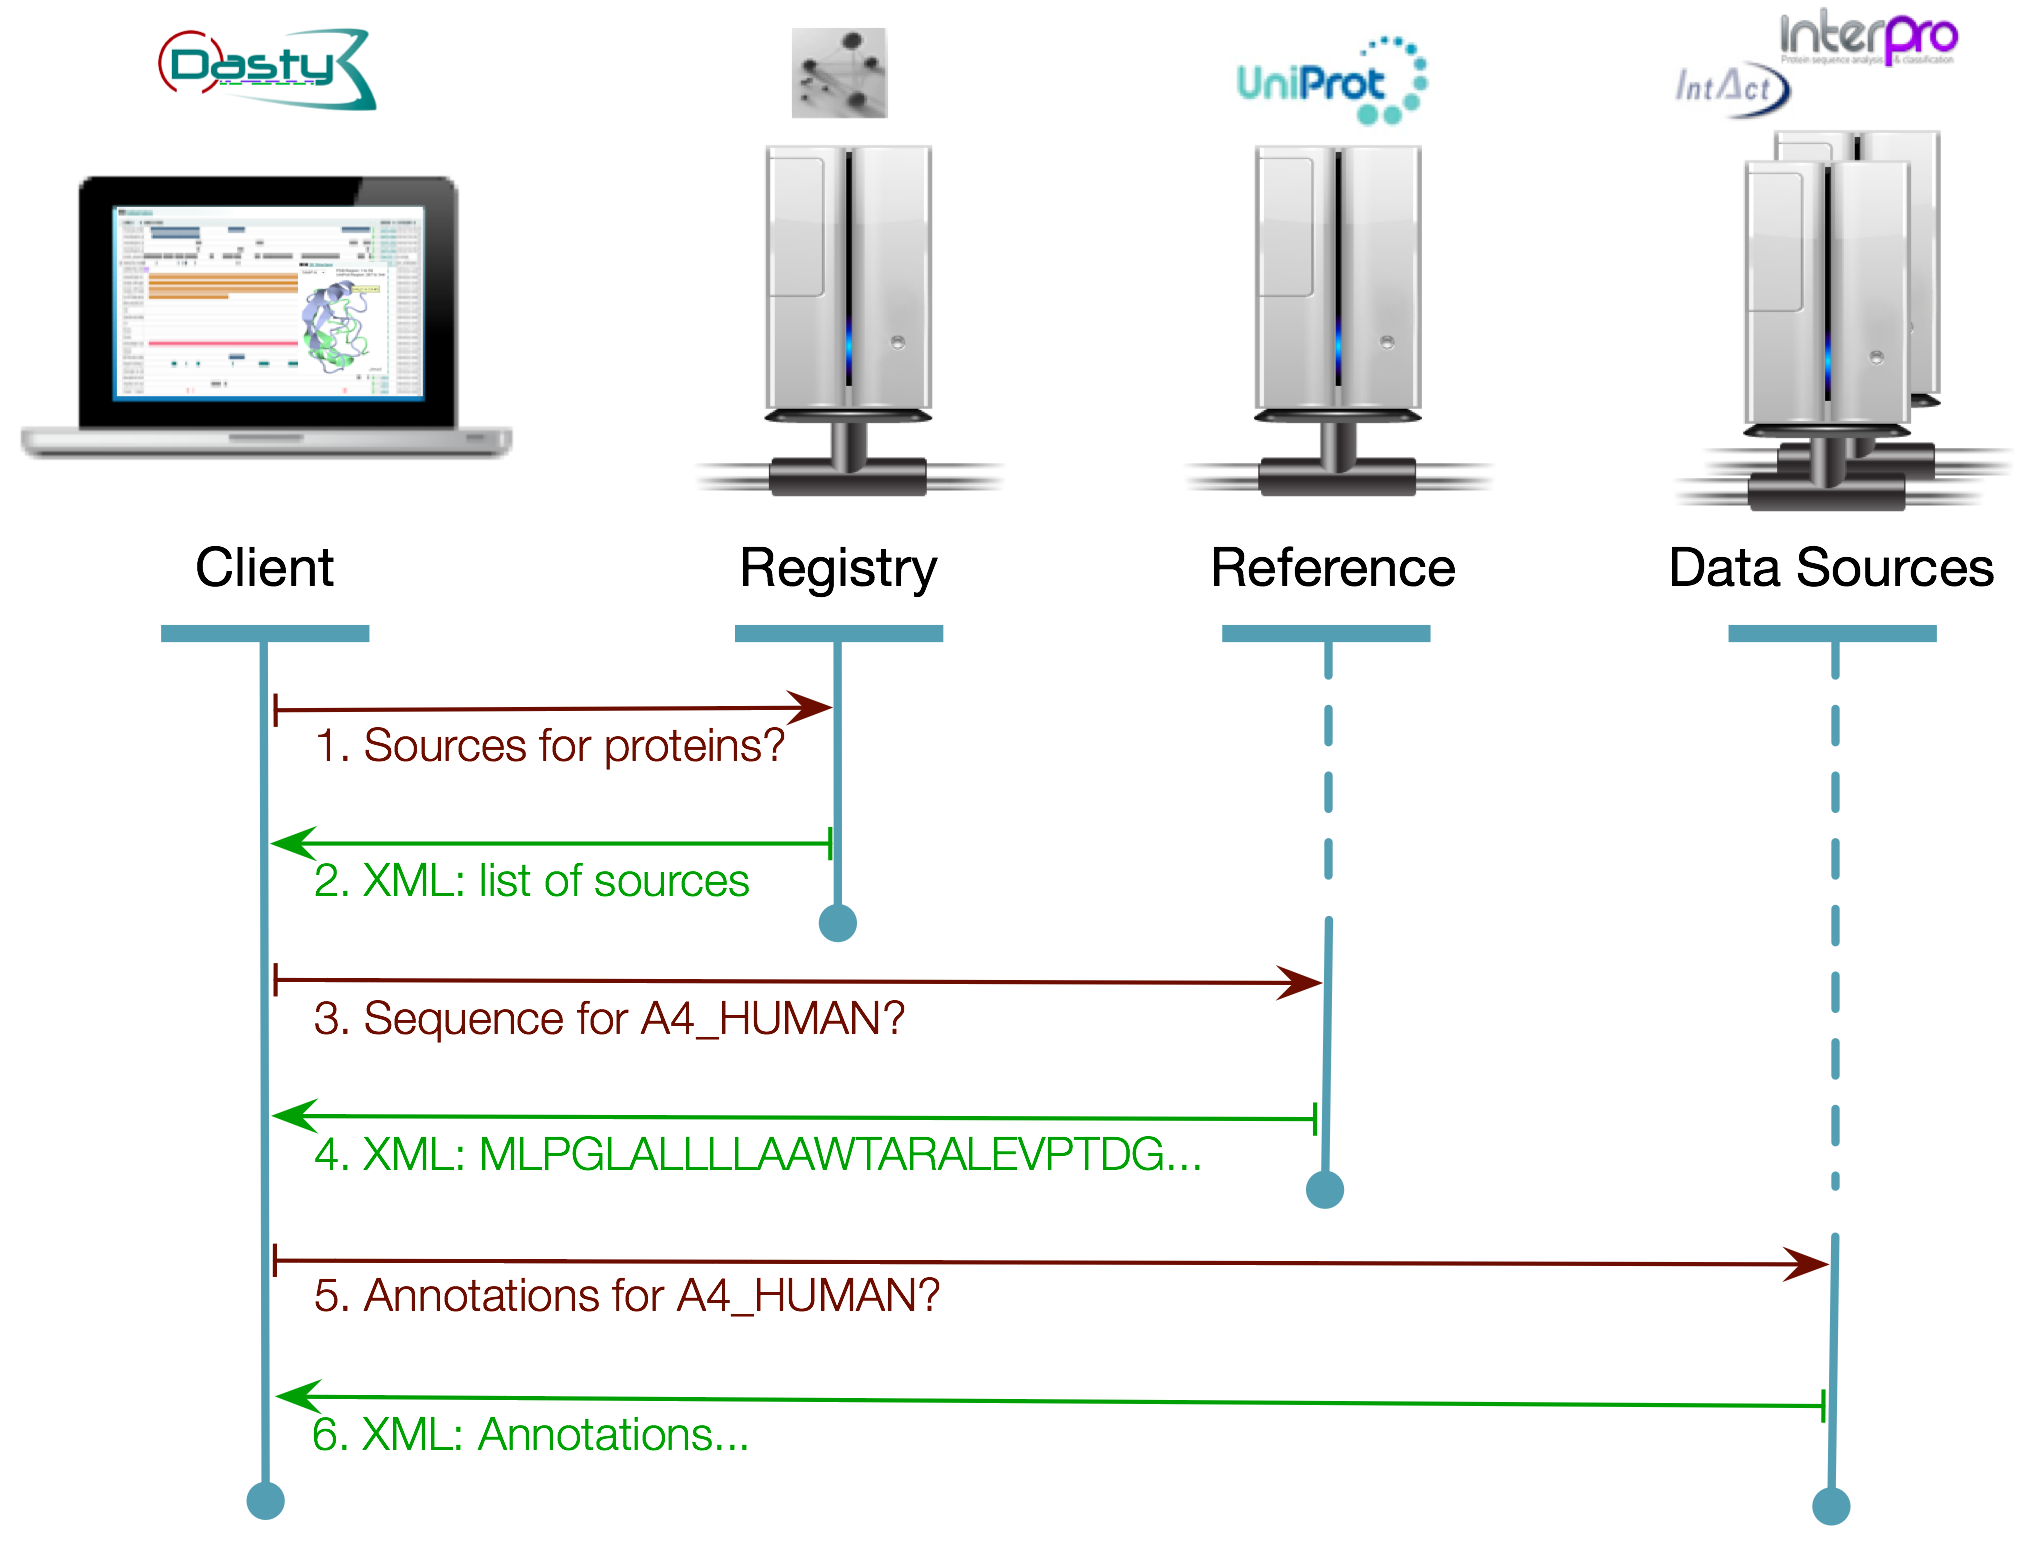
\includegraphics[width=5in]{figures/DAS.png}
\caption[DAS Flow of Information.]{Flow of information in a standard query in the Distributed Annotating System.
\label{fig:das}}
\end{figure}

A regular flow of information in DAS is shown in Figure \ref{fig:das}. The DAS client requests information about a protein that can be specified by its accession or identifier. The client then communicates with the DAS registry in order to retrieve a list of available sources providing information about that biological product. Once the client has retrieved this list, it proceeds to query the DAS reference source, i.e. a DAS source providing the sequence or structure of each molecule that it describes -- UniProt in the case of proteins. The DAS reference source supplies not only the sequence but also meta-data such as the version. Thus clients can ascertain which retrieved annotations correspond to the original request. At this point, the client retrieves features, i.e. annotations, from the available DAS sources. These annotations may be applicable to specific subsections of the sequence (e.g. the location of active sites or observed peptides) or may be applicable to the entire sequence (e.g. related publications or taxonomy). Finally, the client organises and displays the annotations \cite{SAL2010}. 

All these interactions follow an adaptation of the REST protocol for web services \cite{PRL2007} .

\subsubsection{DAS Protocol}
\label{ssec:DASprotocol}
The DAS specification consists of a set of rules which define a standard communication method between the different components of the system. DAS is Web-based and makes extensive use of three widely-adopted standards: the Unified Resource Locator URL, the HyperText Transfer Protocol HTTP and the eXtended Markup Language XML. All communication occurs through HTTP; the requests are URLs that specify the resource that the client is interested in, and the responses are both HTTP codes and XML documents. The details of what constitutes a valid URL, and the XML structure, are contained in the DAS specification.

By the time the first paper about DAS was published \cite{DOW2001}, the DAS protocol was version 1.01, and the main characteristics, such as the \emph{features} and \emph{dna} commands of DAS, were present in that version. From that point, several versions were released with minimal changes. These subsequent versions mostly just polished details to make the protocol stable and useful. The last official release of DAS was Version 1.53 on March 21 of 2002. This was the official version for several years, but in 2006 a new version appeared (version 1.53E) incorporating several new developments. These included an extension to serve new data types and an ontology for protein features \cite{JEN2008}. The E in the version number is for Extended, which essentially describes the purpose of this version, because it keeps most of the features present in 1.53 but extends these to provide some new capabilities.

In November 2007, a project that aimed to define a completely new specification for the DAS protocol was concluded. The new specification was called DAS 2.0 (\url{http://biodas.org/documents/das2/das2\_protocol.html}) and it contained a redefinition of the protocol for the capabilities that DAS had in its previous versions (1.0, 1.53). It also defined new features which allowed for the use of the protocol in a more extensive way. A controversial topic in the DAS community was whether or not the DAS2.0 protocol should be adopted. This specification contains several improvements to the DAS protocol, but given the drastic changes in the format, amongst other reasons, most of the sources decided to continue using DAS1.53 or 1.53E. After the 2009 DAS workshop, it was generally agreed that most of the useful additional features that 2.0 provides would shortly be implemented in DAS 1.6E and its subsequent incarnations. As a result, DAS2.0 is now considered by many to be redundant. Figure \ref{fig:dasevolution} represents the evolution between the various version of DAS, and serves as a comparison between DAS 2.0 and 1.53E/1.6E in terms of number of sources, which is a good indicator of its adoption.

\begin{figure}  
\centering
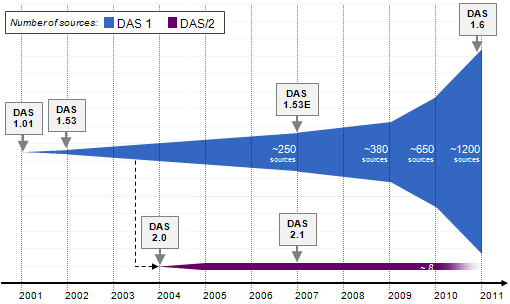
\includegraphics[width=4in]{figures/DasEvolution2.PNG}
\caption[DAS Evolution.]{DAS Evolution.
\label{fig:dasevolution}}
\end{figure}

Version 1.53 of DAS defines the element \emph{FEATURE} as the annotation itself, and it is contained in the element \emph{SEGMENT} indicating that a feature annotates a specific segment, where a segment is a biological residue (or part of it), such as, proteins, genes, chromosomes, etc.

In the scope of proteins, annotations can indicate information about the structure (known formations of amino acids such as helices or sheets), interaction zones (with other proteins or regions of the same protein), phenotype (for example a known relation of part of the protein with a disease), etc. 

An effort to group and organize all the types of annotations has been made: the Biosapiens Ontology contains, in a hierarchical structure, the types of annotations that can be used. As with any ontology, the information is not complete and periodic releases are made trying to establish a set of types as efficiently as possible.  \emph{TYPE} is probably the most important element included in a \emph{FEATURE}. The use of the Ontology is highly recommended but is not mandatory, in order to comply with older releases. 

The use of a second ontology (Evidence Code) is also recommended in the attribute \emph{category} to express the method through which such an annotation was acquired, for instance by experiment, by \emph{in-silico} analysis, etc.

Relevant information for proteins included in the element \emph{FEATURE} is registered in:

\begin{itemize}
\setlength\itemsep{-0.3em}
 \item \emph{id:} A source can not have two features with the same id.
 \item \emph{label:} A human readable label for the feature
 \item \emph{START} and \emph{STOP}: Indicating the specific position to be annotated. If both are equal to zero, it means that the annotation applies to the whole segment (i.e. \emph{Non-positional feature})
 \item \emph{LINK}: To indicate a URL where more information about this annotation can be found.
 \item \emph{NOTE}: Space where the annotator can add any extra comment about the annotation.
\end{itemize}

Other elements and attributes are more oriented to other kinds of biological data, for instance the \emph{ORIENTATION} element is useful for genes, to indicate if the annotation follows the direction 3' or 5', however proteins do not have an orientation.

DAS can be seen as having a \emph{``Dumb server -- Smart Client''} architecture where most of the hard work is executed in the client. Nonetheless, several independent projects have contributed to both clients and servers. 

Under the DAS terminology, servers and sources represent two different concepts. A \emph{DAS source} provides data for one \emph{Coordinate system} (\url{http://www.dasregistry.org/help_coordsys.jsp}), i.e. a unique 4-tuple \emph{(Authority, Version, Type, Organism)}, e.g. (Ensmbl, 51, Chromosome, Homo Sapiens). On the other hand a \emph{DAS server} is the software that facilitates the publishing of DAS sources.

Each DAS source can support several capabilities, which means it is able to respond to an HTTP request that gets interpreted as a DAS command (e.g. sequence, features) with a document that follows the specification. DAS servers are pieces of software that implement the common tasks of this process, for example handling the HTTP requests, providing a logical model for DAS or encoding the model into a document.

The two most representative implementations of a DAS server are Pro-server \cite{FIN2007} and MyDas \cite{SAL2012}. Both have been updated to support the latest version of the specification (i.e. 1.6E) and their feature sets are similar. Probably the biggest factor in choosing between these two implementations is the preference for a particular programming language: Perl for Pro-server and Java for MyDas. An extended description of MyDas can be found in the section \ref{section:mydas}, including the contributions to MyDas as part of this PhD project.

On the other side of the spectrum, the DAS clients have the task of providing a unified view of multiple sources. Most of the DAS clients centered their efforts on a particular DAS type, such as proteins (e.g. DASher \cite{MES2009}), chromosome (e.g. Ensembl viewer \cite{FLI2011}) and genomes (e.g. Dalliance \cite{DOW2011}), where others such as SPICE provide a way to navigate between multiple DAS domains. For instance, it is possible in SPICE to start on a chromosome view, zoom-in into a gene region, select the expressed protein of the gene and visualize its 3D structure, all in the same Java Web-start window \cite{PRL2005}.

Dasty2 is a Web client that also supports the interaction between protein data and its 3D structure, but its current version doesn't support direct manipulation of genomic data \cite{JIM2008}. A refactoring of Dasty was executed during 2010 and is explained in detail in section \ref{section:dasty}, including our contribution to the effort of developing Dasty3 \cite{VIL2011}. 

\subsection{Discussion}
Besides the primary data from \emph{in-vitro} experiments, there are hundreds of secondary sources consolidating data that results from \emph{in-silico} analysis. All the projects mentioned contribute in different ways to the creation of a pool of knowledge where both primary and secondary sources are available to the researchers.

Some of these projects started when a problem was detected while trying to compile the generated data of a particular community (e.g. BioPAX); while others have studied an existing technology such as data warehouses, web services or semantic web and proposed adaptations to it for bioinformatics needs (e.g. Biowarehouse, BioMoby). Some approaches are on the protocol and specification level (e.g. SADI) while others take existing specifications and generate the tools to facilitate their implementations (e.g. BioRDF). There are projects that take existing software and adapt it to bioinformatics (e.g. WikiPathways) and others develop completely new software (e.g BioMart, Taverna). Some focus on the integration of the data (e.g. BioMart) and others on the interconnections between components (e.g. Galaxy). Some focuses on the tools (e.g. SRS) and others on the results and their publications (e.g. WikiGenes). 

Despite their origin, methods, technologies or approaches; all of these projects have in common the need for a strong community that supports its development, maintenance and use. We chose DAS as the base technology on which our contributions will be focused because when we started the project, it had a growing community as seen in figure \ref{fig:dasevolution}. It was based on existing and consolidated technologies such as the HTTP protocol and REST services, and it had the support of big entities and projects, such as the EBI and Ensembl. A description of the specifications and software components developed as part of this PhD project can be found in chapter \ref{section:integration} of this document.

\newpage


\section{Visualisation}

The field of visualisation aims to represent data in such a way that non evident features become visible. The techniques developed to achieve this objective vary from simple ones (e.g. histograms) to very elaborate (e.g. environments only visible using 3D virtual reality rooms).

The uses of visualisation techniques are as diverse as the fields in which they are used, from weather forecasts in the news to the analysis of the data captured in the Large Hadron Collider. In our field of interest, bioinformatics, the use of visualisation methods is also abundant, and sub-fields such as genomics, proteomics, population variance, etc. have plenty of examples where different techniques have been implemented with the purpose of making sense of biological data via visual representations.

The most representative visualisation techniques used in bioinformatics can be categorised into three groups: charts, networks and hierarchies. Charts are graphical representations where n-dimensional data is mapped or aggregated into a space, for example scatter plots, bar graphs, pie charts, etc. Networks are structures where some components are connected to an arbitrary number of other components, normally using a node-link metaphor where the components are represented by nodes and the connections are lines between them. Lastly, hierarchies are another type of connection that show when an item is part of another, or using graph theory terminology: a node can be the parent of another. The diverse representations of trees can be used for this type of data, for example, node-link trees and space filling diagrams \cite{WAN2014}. 

\begin{figure}  
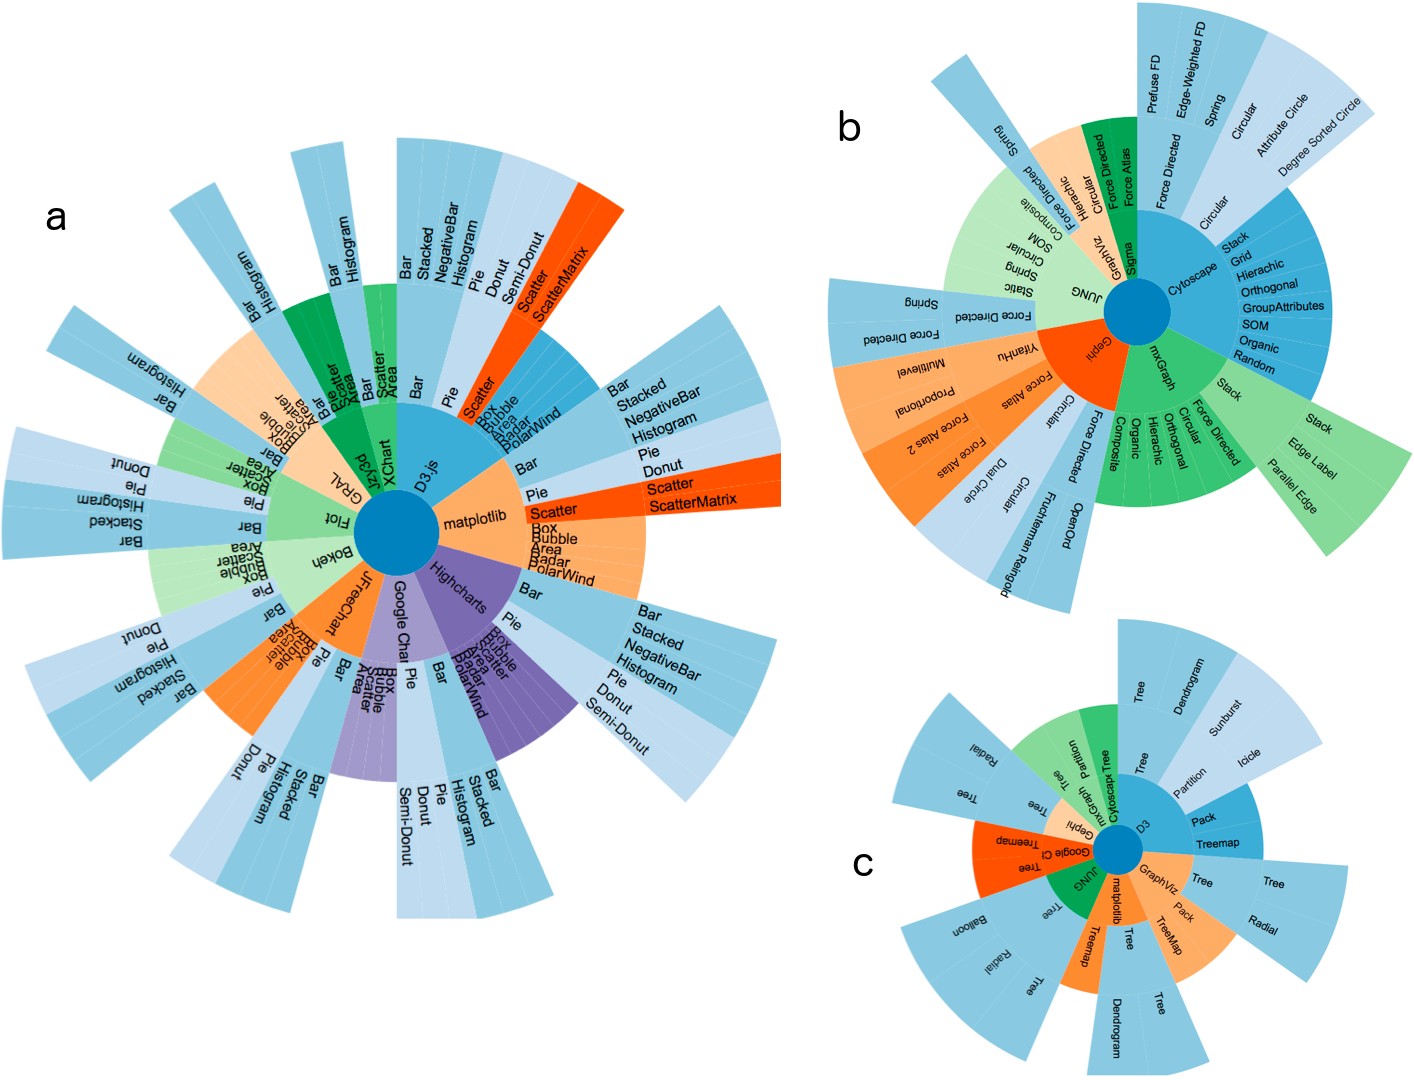
\includegraphics[height=6in,angle=90]{figures/vis_libs.png}
\caption[Comparison of features of selected visualisation libraries.]{Comparison of features of selected visualisation libraries grouped by their support of (a) charts, (b) networks and (c) hierarchical representations.
\label{fig:vis_libs}}
\end{figure}

Figure \ref{fig:vis_libs} shows a comparison of several libraries that have been used in bioinformatics research \cite{WAN2014}. The libraries in (a) include the capability to represent charts, while (b) and (c) show similar graphics for libraries that support network and hierarchical representations respectively. It is worth noting that several libraries are present in all three graphics because they have been developed without a specific domain in mind so that they can be useful in a variety of applications.
 
A recurrent challenge when visualizing data is to match the most appropriate combination of techniques to the nature of the data, optimising the features of the visualisation (e.g. location, colour, size or shape) in order to highlight a biological characteristic (e.g. genomic position, functional class, expression level or organism). As stated in \cite{GEH2010} ``\emph{The challenge is to create clear, meaningful and integrated visualisations that give biological insight, without being overwhelmed by the intrinsic complexity of the data}''.

A variety of projects in different subdomains of bioinformatics have been presenting alternatives according to the needs of each case. The sections below describe some of the most illustrative projects, grouped by some well known bioinformatics domains.

\subsection{Genomics}
Genomics is arguably the subfield that produces the most abundant, basic and yet relevant type of data in molecular biology research. Advances in the methods for extracting and interrogating DNA, RNA and other biological products have grown dramatically in recent years. For example, sequencing projects have progressed from taking decades to gather the approximately 3.3 billion base-pairs \emph{bp} of the human genome, to the ability to extract over a billion short reads (i.e. individual sequences of approximately 100bp) in days or even hours with some of the new technologies known as Next Generation Sequencing (NGS).

This comparison may, however, be unfair because the number of reads produced by NGS still requires a large amount of processing in order to assemble a genome because it is more challenging to align NGS short reads than the reads from first generation sequencing, however this extra processing time is in the order of days or weeks, not the years required previously. 
%Moreover, none of the NGS technologies would have been possible without the findings of the human genome project. 
Nonetheless the comparison still serves to reflect the rapid development in the methods of sequencing DNA.

Visualisations have played an important role in the different stages of genomic analysis. In \cite{NIE2010}, the authors have identified three tasks in genomic's research where visualisations have been widely used: (i) supporting the sequencing process, (ii) browsing annotations in the context of a reference genome, and (iii) comparing sequences from different organisms and/or individuals.

\subsubsection{Sequencing Process}
Despite all the progress in sequencing techniques, the process is not perfect and requires visual inspection in order to interpret and validate automated outputs to compose sequences, chromosomes and ultimately genomes. It is a common strategy to associate quality scores (QS) to each of the nucleic acid bases that result from a sequencing experiment. The QS is proportional to the number of agreeing reads that cover a base. For example the QS on a given position X would be low if half the reads covering X indicate a G and the rest point to a T. It would be similarly low if only few reads cover that area or if the bases are not clearly distinguished in the reads. In contrast, if many reads are covering an area and all of them agree to assign A at X, the score in that position would be high.

Several tools have been developed which take advantage of this information to align the reads and represent the scores in multiple ways. For example histograms or heat maps ease the task of identifying regions of low coverage and expose errors in the automatic consensus sequence. This type of tool is highly dependent on the technology used. For instance, there are no raw read traces (only images) in some of the NGS techniques, and therefore a detailed alignment view that includes the images corresponding to each read is computationally expensive, and consequently, some tools do not support that level of detail. 

Some of the read alignment viewer tools go beyond the display functionalities to allow editing of the assembly in order to complement the automatic result and to annotate relevant parts of the sequence (e.g. genes, promotors, etc).

HawkEye was one of the pioneering tools that offered some of the features discussed above, and mainly focussed assisting with the detection and correction of assembly errors for whole-genome shotgun projects \cite{SCH2007}. This stand-alone tool offers a Top-Down strategy to analyse an automatically assembled genome. Figure \ref{fig:hawkeye} presents the three main views included in Hawkeye: 

\begin{description}
\item[(a) The launch pad] is the first screen presented to the user when a draft genome has been loaded. It acts as a global overview by displaying summary assembly statistics in the form of two N-Plots (i.e. A bar graph where each bar is a container). Its height represents the length of the container in bp, and the width its length in percentage of the genome size.
\item[(b) The Scaffold View] represents the current scaffold as a linear ordering of connected contigs, with the assembly features displayed below. The first two tracks are heat map plots to easily visualize the insert and read depth coverage. This view allows zooming and panning in order to navigate through the assembly.
\item[(c) The Contig View] follows the same design as the scaffold view by representing the consensus on top and the composing items aligned below, however in this case the level of detail can be expanded to show the nucleotide bases along with their quality scores and the chromatogram traces when available.
\end{description}

\begin{figure}  
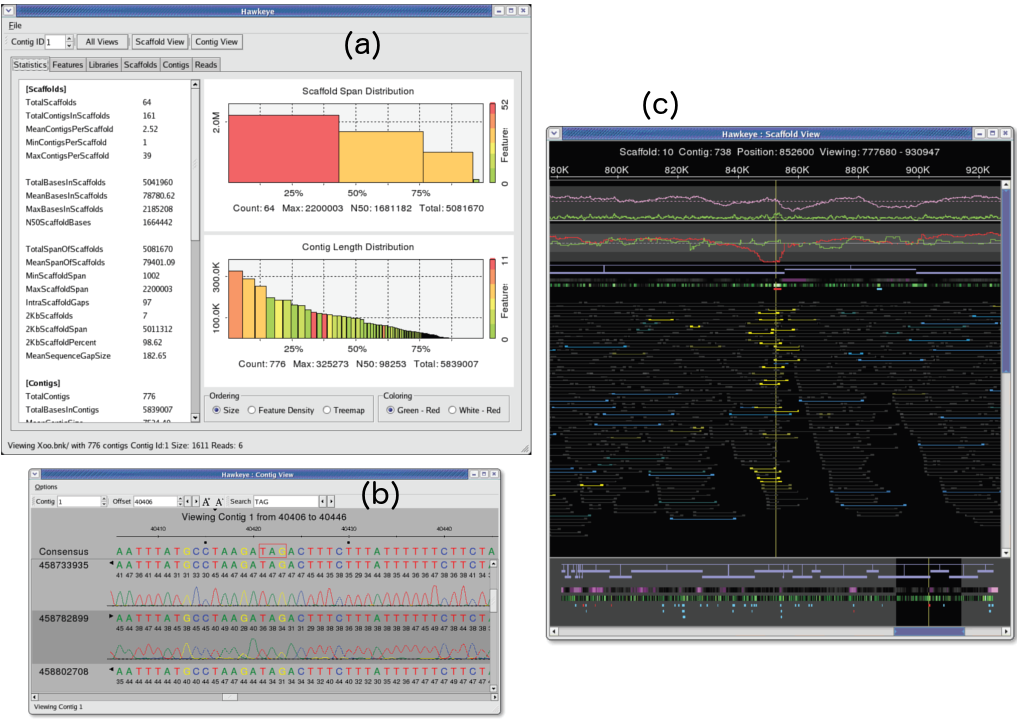
\includegraphics[height=5.7in,angle=90]{figures/hawkeye.png}
\caption[Hawkeye Interface Views.]{Snapshots of the available views in the Hawkeye tool: (a) Launch Pad, (b) Scaffold View and (c) Contig View.
\label{fig:hawkeye}}
\end{figure}

The formats to store read alignment information have been influenced by the technical changes imposed by the new technologies associated with NGS. The SAM format was created as part of the 1000 Genomes project \cite{GEN2012} as an attempt to provide a generic alignment format that supports single and paired reads. A SAM file can then been converted to BAM, which is a binary lossless compressed file that can be indexed to offer rapid access to a specific position on the alignment \cite{HEN2009}. 

A set of tools called SAMtools was developed by the same team in order to help with the basic operations required to manipulate a SAM file. It includes a Text Alignment Viewer, which, despite being very basic and command line based, is of great help to researchers because its simplicity results in high performance, which makes the navigation of full genomes very fast.

Similar formats to SAM have been developed around the NGS technologies in order to store different types of data, for instance, BigBed and BigWig, which are the Big Binary Indexed (BBI) versions of the BED and WIG formats. BED files are used for tables with a varying number of fields, where each line contains the fields for one record separated by a white space. WIG files are used to associate a double value to each base. This format is designed to compress information when the same value is assigned to a large section of the sequence \cite{KEN2010}.

The Integrative Genomics Viewer (IGV) is one of the tools that takes advantage of these new formats to enable real time exploration of large-scale genomic data-sets at different resolution scales \cite{ROB2011}. Data sets of both basic aligned read sets as well as deviating results can be loaded into IGV from local and remote sources. IGV can then be used to detect and correct assembly errors such as misalignments in repeat regions. IGV also supports the display of annotation files in the context of the genome, making it suitable for the category (ii) defined at the beginning of this section.

A description of other tools that support the process of sequencing a genome (category (i)) can be found in \cite{NIE2010}. Once the genome is ready and has been through a finishing process, it is usually shared and other scientists can use it in the context of their own data. It is at this stage where the tools of category (ii) i.e. browsing a completed genome with its annotations; are of great help.

\subsubsection{Genome Browsing}
A famous principle in visualisation is known as the Shneiderman mantra: \emph{overview, zoom, filter, details-on-demand} \cite{SHN1996}. Most genome browsers use a similar layout that follows the mantra quite closely, adapting it to the molecular biology behind the data.

The \emph{overview} is usually a graphical representation of the karyotype, which is the set of chromosomes displaying its bands. The bands have been experimentally defined using cytogenetics techniques to identify parts of the chromosome, and are used as visual markers for different chromosomal regions.

The user can \emph{zoom} into a chromosome band, or can select a region of interest by interactively marking an area, or by explicitly introducing the coordinates. Once a region of interest (ROI) is selected, a multi-row visualisation is displayed, where the first row represents the ROI. Some browsers use colour coding for this row to show the limits of the bands or other high level features of the region.

Each subsequent row is called a track and displays a different set of features drawn proportional to the selected region. For instance, it is common to include a track displaying the annotated genes in the ROI, using boxes to represent exons, and lines for introns. Other symbols can be used to represent different features, e.g. arrows to define if the gene gets translated in the direction 5' to 3' or the other way around (reverse strand), or colours can be used to represent the functional class of the gene, etc.

Most genome browser have a wide list of sources that provide different types of information such as transcription factor, binding sites, single nucleotide polymorphisms (SNPs), details about the sequencing source (e.g. contigs, reads), proteins, supporting evidence, etc. The tracks to be included in the browser are then selected and \emph{filtered} by the user. 

Finally a feature of interest can be selected to obtain \emph{details-on-demand}, for instance, to get a link to a website that contains the information about the protein encoded by the selected gene, or specific data on the allele frequency of a SNP and its associated phenotype.

\begin{figure}  
\centering
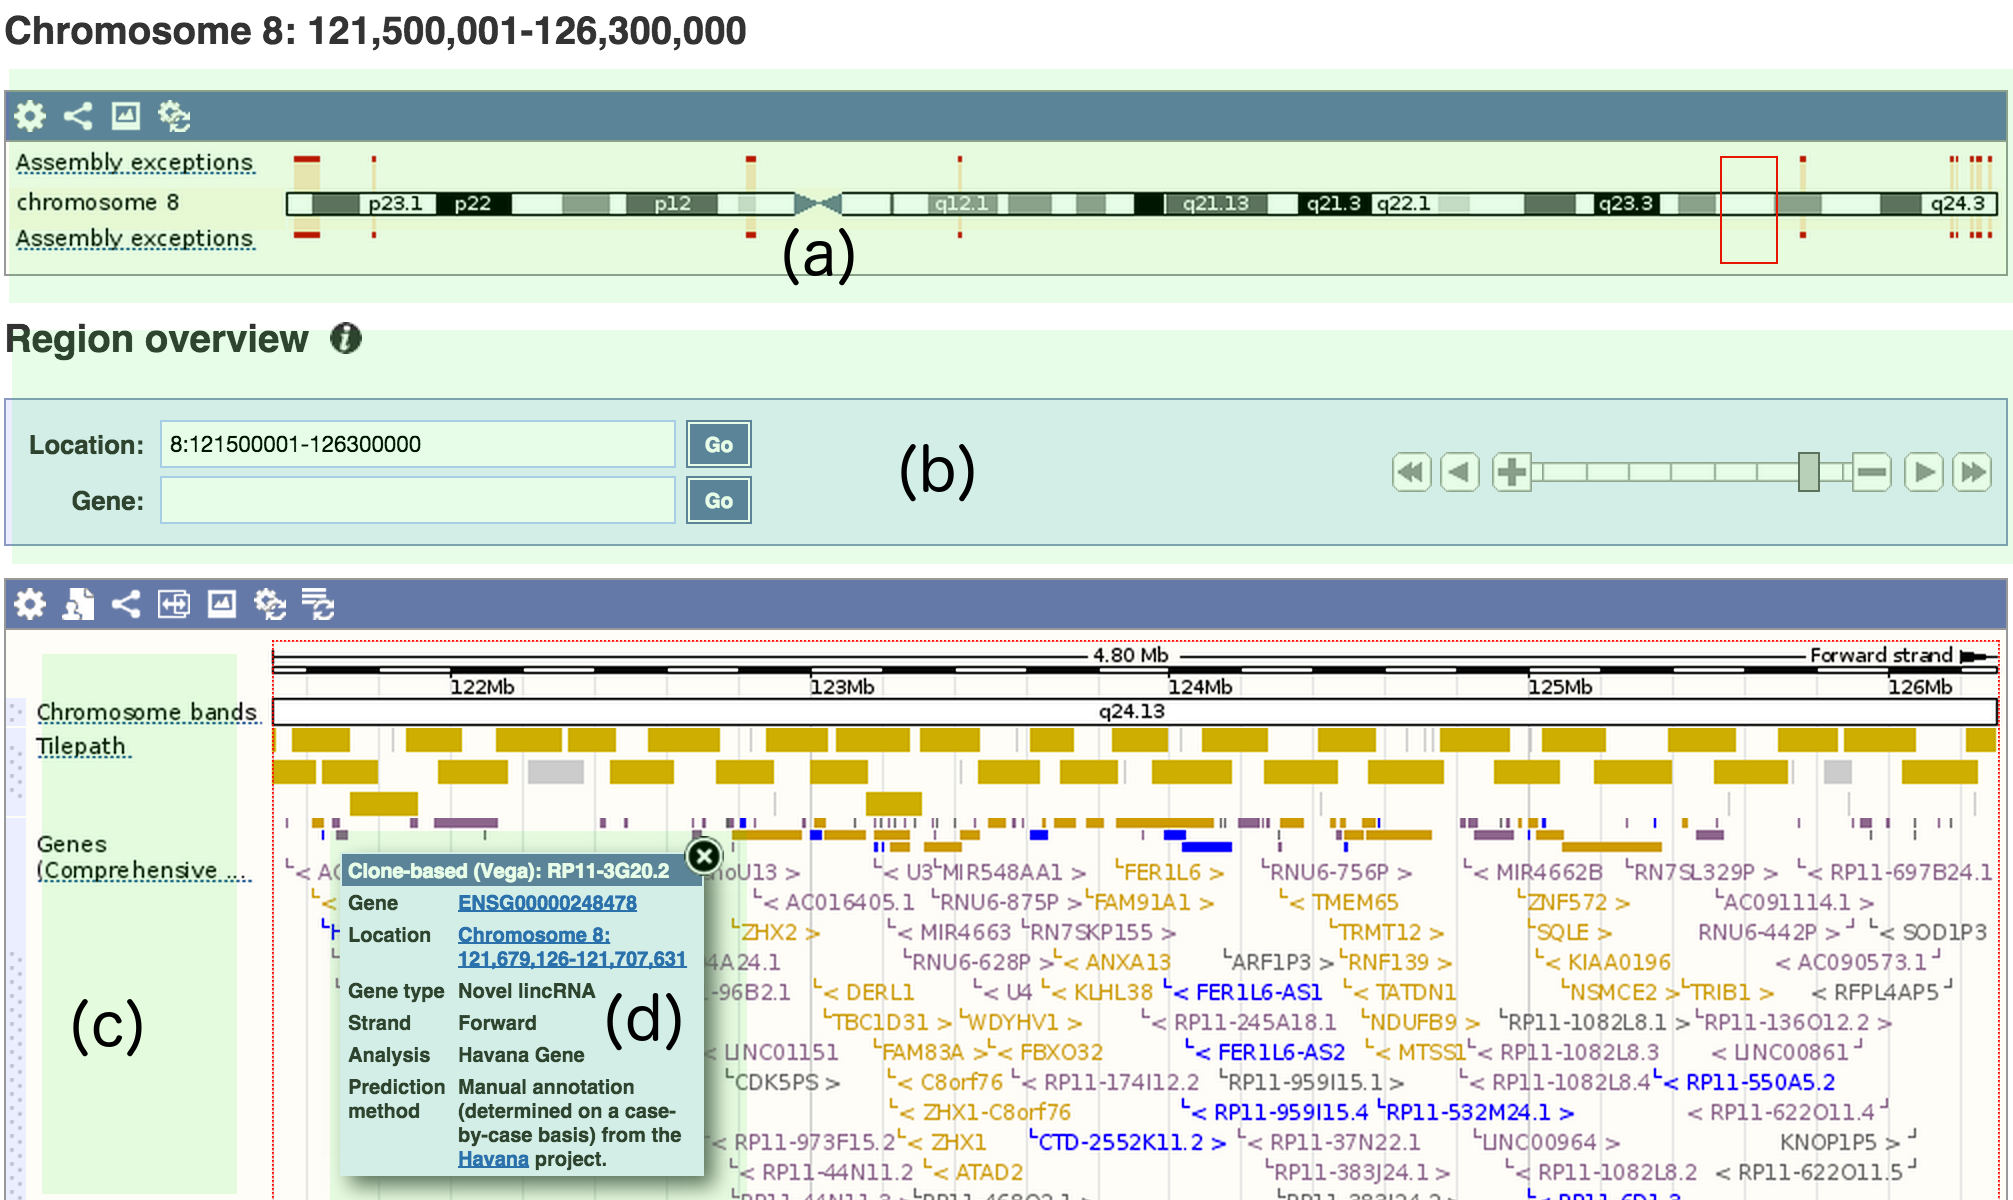
\includegraphics[width=\textwidth]{figures/ensembl_snapshot.png}
\caption[Snapshot of the Emsembl genome browser.]{Snapshot of the Emsembl genome browser highlighting the components that support the implementation of Shneiderman mantra: overview(a), zoom(b), filter(c), details-on-demand(d).
\label{fig:ensembl_sn}}
\end{figure}

Figure \ref{fig:ensembl_sn} shows some of the widgets used by the Ensembl genome browser that follow the Shneiderman mantra. Region (a) displays a selected chromosome showing the overview of the data, in (b) it is possible to select the zoom level and the coordinates to mark the ROI; (c) shows the name of the sources that have been selected for the current graphic, and (d) is a pop-up window displayed when the user clicks on one of the features of the graphic.

The Ensembl website (\url{http://www.ensembl.org/}) aggregates all the information that has been integrated through the Ensembl project. The dataset has grown from having partial information in 1999 for one species: \emph{Homo Sapiens}; to include full support for 69 species by the time of the release of version 77 in October 2014. 

From the beginning, the objective of the Ensembl genome viewer was to support multiple species with a single software installation. The challenge goes further than the amount of data generated by species, because there are many differences in the data from one species to another \cite{STA2004}. The project has clearly been successful, not only judging by the number of species included, but more importantly because of the size of its community, reflected by more than 1500 user queries assisted by their helpdesk team in 2014 \cite{CUN2014}.

Besides the sources provided by Ensembl, it is also possible to include external sources by using several protocols. For example, it is possible to include a URL to several NGS files (e.g. BAM, BigBed, etc.), or to point to an existing data source that uses the DAS protocol (discussed in section \ref{ssec:DASprotocol}). With this information, Ensembl will query that source to get information on the ROI and display it in location views, such as the Region in detail, chromosome or karyotype view. Moreover, Ensembl is in itself a DAS source, which makes it easy to include Ensembl data in other resources \cite{SPU2010}.

Similar efforts to Ensembl have been addressed by two other big organizations: the NCBI Map Viewer \cite{ACL2014} and the UCSC Genome Browser \cite{ROS2014}. Both projects provide easy access to the centralised repositories of each institution, and allow third party data to be displayed in the context of their own data. Moreover, they collaborate with each other, and information from one source is available for display on the other. A comparison between these three genome browsers can be found in \cite{FUR2006}.

These traditional genome browsers share the same architecture, where both data and services are located on the server side: when a new request arrives, the data is collected from local or third-party data sources, and then an image is created by the server, which is ultimately transmitted to the client; HTML link-maps are also generated to include interactive links over the image. In this way the client only requires the ability to display images and the use of the \emph{map} HTML element, which has been part of the HTML specification since early versions, and therefore is widely supported.

Unfortunately in using this approach, it is necessary to re-generate a completely new image with most user interactions, for example, by moving the ROI by a few bases, or by hiding a data source. Some strategies have been developed to improve the usability of these applications, for instance using cache memory in the server to accelerate the access to remote sources, or pre-generate the most likely required images (e.g. left and right of the current region). Nonetheless, factors such as the number of sources or network delays can dramatically affect the smoothness of the navigation in a system of this type.

Recent web technologies permit the decentralisation of the data, increasing the workload on the client and therefore liberating the server from most of the display related tasks. According to this model, the web genome browser is an application that mainly runs on the client, requesting data on-demand and generating/manipulating the graphic accordingly. If, for example, the user drags the display area to the right, making a few more bases visible, the client only requests the information of the new area, and alters the graphic dynamically. This reduces the computational cost of creating a full image, but most importantly isolates all the ``look and feel'' tasks from the server, allowing the server to focus on serving data, and consequently to attend to more and bigger requests.

JBrowse is an open source application that follows this approach implementing a robust client in JavaScript with the support of a server side developed in Perl for the preprocessing of the data. JBrowse uses a combination of standard HTML 'div' and 'canvas' elements to represent the genomic features. For instance in high level views of data, 'divs' are used to create histograms to show the number of features in an area. As in the case of other genome browsers, JBrowse supports the inclusion of third-party data using NGS files. For example, BigWig data is represented either as heat maps or histograms using 'canvas' elements \cite{LEE2013}.

There is another strategy for genome browsing, which takes advantage of the features of what is also known as Rich Internet Applications (RIA). This preprocesses the information to create small images called tiles that can be used to compose a view, similar to the experience introduced by Google maps; in this way there is no need to refresh a whole page if there are minor changes in the selected area. 

However, in \cite{SKI2009} the authors of JBrowse present a benchmarking experiment, where the two approaches are tested. The results of the experiment show better response times in the case where they used HTML elements. Besides the performance, the 'tiles' approach requires a lot more storage space in order to have all the tiles pre-calculated, moreover, the approach complicates the desirable features of including third-party sources because it might need to pre-process the entire source to create the tiles.

A similar project to JBrowse is Dalliance, a Web-based Genome Viewer developed using the HTML5 capabilities to manipulate SVG elements. It also requires a modern web browser (Firefox 3.6+, Chrome 5+, Safari+). Dalliance takes advantage of the DAS architecture in order to allow the users to put custom data in the context of reference genomes. As with other genome browsers mentioned above, it supports the interaction with BAM files and other NGS related formats \cite{DOW2011}. 

Similarly MyKaryoView uses DAS in order to include other sources, this tool places special emphasis on the display of personal genome data in context with well known data sources \cite{JIM2011}.

It is important to highlight that the purpose of genome browsers is to simplify the task of generating hypotheses based on the aggregation of genomic data. Each data source can contain errors, and the researcher should be sceptical of any conclusion based on a single observation. Genome browsers allow the graphical display of several sources, and in this way make it easier to detect anomalies, errors or special genomic conditions. Despite how evident a hypothesis is represented in a visualisation, the scientist must have access to the original data in order to evaluate any theory \cite{CLI2009}.

\subsubsection{Comparative Genomics}
The last of the categories (iii) mentioned at the beginning of this section, refers to the group of tools used to compare genomes between individuals and/or species.

With the constantly growing number of complete genomes, it is a logical step in research to look for high level similarities between them and to use the knowledge discovered for one species for the research of others. This field, known as comparative genomics, tries to identify functional elements common in multiple species and their evolutionary origins. It is also common to use these techniques to assist in the assembly and finishing of new genomes.

The estimation of the conservation of chromosomal location of multiple genes among several species is known as synteny. Its relevance lies in the assumption that a sequence of genes in the same location in two species is an indication of a common ancestor. A "dot plot" graphic (see Figure \ref{fig:dotplot}) is commonly used to represent the synteny between two genomes. Each of the two dimensional axes of the plot represent one of the genomes, and dots in the graph are the positions where a common gene is located. Connected dots that show a 45 degree line are an indication of a highly syntenic region. Tools such as Vista \cite{FRA2004} and GenomeMatcher \cite{OHT2008} include implementations of dot plots along with other ways to compare genomes.

\begin{figure}  
\centering
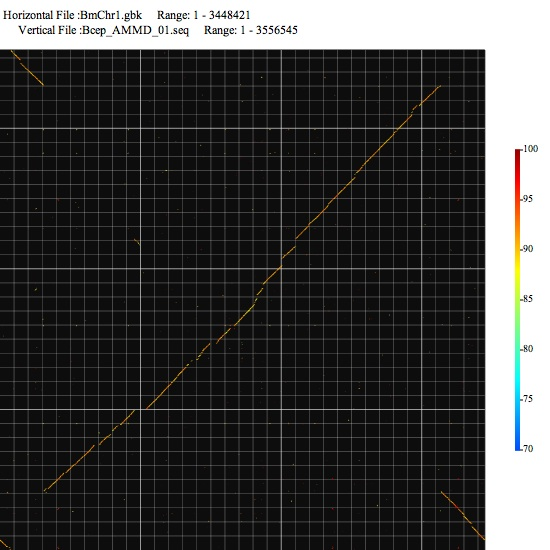
\includegraphics[width=4in]{figures/dotplot.jpg}
\caption[Dot plot comparison created with GenomeMatcher.]{Dot plot comparison created with GenomeMatcher
\label{fig:dotplot}}
\end{figure}

As an alternative to dot plots, some tools offer a technique to display multiple genome alignments and mark corresponding areas between them by colour-shadowing. For example, Figure \ref{fig:gbrowsesyn} shows an example generated using GBrowse\_syn \cite{MCK2010} where multiple genomes from the WormBase database have been aligned and a section is displayed to show the conservation of certain genes.

\begin{figure}  
\centering
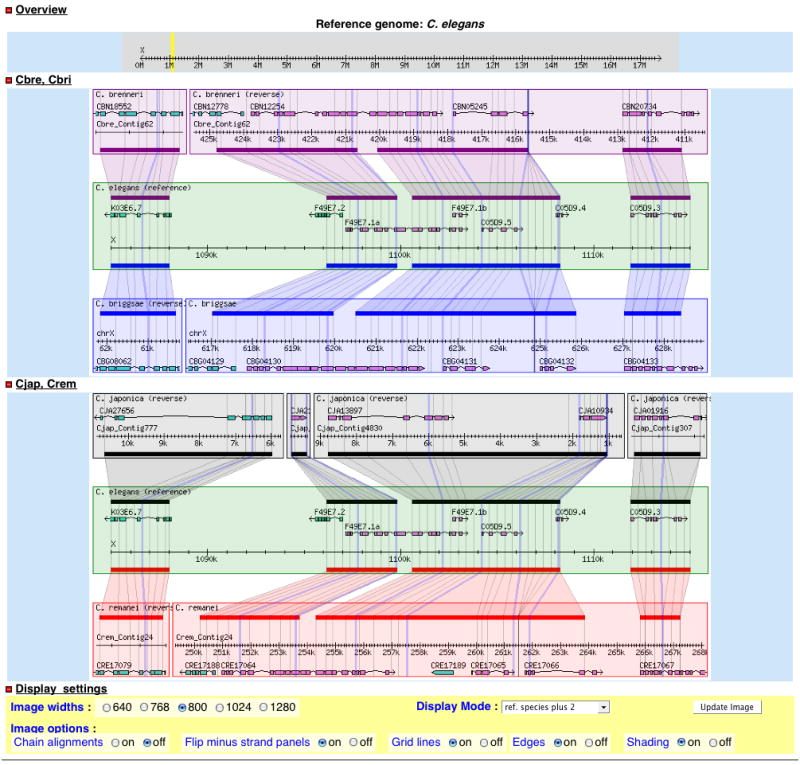
\includegraphics[width=\textwidth]{figures/gbrowse_syn.jpg}
\caption[Multiple alignment snapshot generated with GBrowse\_syn.]{A five species whole genome DNA sequence alignment comparison from WormBase using GBrowse\_syn.
\label{fig:gbrowsesyn}}
\end{figure}

Besides the comparison of genomes between species, the progress of sequencing techniques permits the analysis of multiple individual genomes of the same species in order to study their variation, and, in this way to try to discover the genotype that causes phenotypes of interest, such as diseases. The largest international effort in this area to date is known as the 1000 Genomes project, which at the time of their latest publication \cite{GEN2012} includes the genomes of 1092 individuals from 14 populations, in which they genotyped 38 million SNPs, 1.4 million indels and 14000 large deletions. All of these data provides vital information for genomic studies on human health.

An adaptation of the Ensembl browser has been developed in order to provide a way to visually browse through the resulting information from the 1000 Genomes project. Multiple tracks including aggregates and results from the study have been added to the browser and new functionalities to export and visualise variation data are now part of this tool.

\subsection{Proteomics}
At the central dogma of biology, DNA (deoxyribonucleic acid) encodes genes, which get transcribed into RNA (ribonucleic acid), which in turn, gets translated into proteins. Each of these is represented by a sequence of either nucleotides (DNA, RNA) or amino acids (proteins). In the previous section we discussed the visualisation tools that assist in the processing of DNA sequences in order to get a full genome of a species, where positional annotations can be included, shared and explored in the context of one or multiple organisms. 

It is because of the central dogma that annotations for genes are among the most used and useful features to know about on a DNA sequence. The direct relationship between a gene and a protein is the key to a large part of molecular biology research. For example, many diseases are caused because there are not enough (or too many) proteins to execute a biological function, or because there are proteins but they are malformed. In either of these cases, the source of the problem can sometimes be traced back to the gene that generated the protein, where, for example, a mutation has appeared, or a section of nucleotides have been inserted/deleted (indels). 

It is one of the goals of proteomics, at least in the clinical context, to deliver markers for disease prognosis, state and treatment outcome and targets for disease treatment \cite{MIS2007}. The Online Mendelian Inheritance in Man (OMIM) resource is a catalogue of human genes and genetic disorders \cite{AMB2014}. In OMIM it is possible to find out what mutation in a gene (genotype) is associated with a disease (phenotype). This information has been compiled from peer reviewed publications that represent the current knowledge in the area from several communities (clinicians, molecular biologists and genome scientists). This, of course is a work in continuous progress and despite the enormous contribution of resources such as OMIM, it is not by any means a finished task.

Once a good approximation of the genome of an organism has been determined, deciphering its proteome (i.e. the total protein complement of a cell, organ or even an organism) is the next logical step to take, especially considering that the number of identified genes from the human genome project (\textasciitilde20000) is far too small to explain the complexity of human biology \cite{PAN2008}.

This is due (among other reasons) to gene and protein splicing and post-translational modifications (PTMS), which makes it impossible to completely deduce the proteome from the genome. Therefore, approaches that start at protein identification are necessary in order to study proteins that otherwise wouldn't be detected. Besides, the discovery of genes by computational means is limited and proteomics techniques offer an alternative solution and verification of gene prediction.

Multiple experiments have been developed in order to address this challenge. For example: mass spectrometry (MS) helps to identify which peptides and ultimately which proteins are present in a given sample, and 2D gel electrophoresis and protein microarray analysis can provide insights to the proportions of proteins that have been expressed under certain conditions (e.g. a specific tissue, a sick patient, a healthy person (control), etc.). Similar data can be obtained with alternative uses of NGS technologies such as RNASeq fro gene expression; and crystallography and modelling software have been used to determine the final 3D structure of proteins.

Visualisation has shown its potential by helping in the understanding and analysis of the results of such experiments. Below we will show some cases, grouped by some of the most frequently used proteomics techniques, where visualisation methods have been used to support the analysis.

\subsubsection{Gel Based Proteomics}
Two-dimensional polyacrylamide gel electrophoresis, usually called 2D PAGE  is still the most widely used approach in top-down proteomic studies, mostly due to its efficiency at separating proteins in complex mixtures. Figure \ref{fig:gelflow} presents the usual steps involved in an 2D PAGE experiment that separates the proteins of interest for a particular hypothesis, which can be then identified with, for example, MS techniques \cite{SIL2014}.

The four first stages in this flow describe the preparation and execution of the experiment itself, which results in a set of gels (one per sample) where proteins are separated according to molecular size and isoelectric point. Conglomerations of proteins are then exposed as darker spots. In order to analyse the relevance of the different proteins to the hypothesis of the particular study, the gels need to be digitised and processed, quantifying the protein concentration on each of the detected spots (alternatively some techniques quantify per pixel). Multiple techniques of image processing are applied in order to clean and extract the data, then normalisation and stabilisation is executed. The output of this process is a matrix in which every row represents a sample, and every column represents a spot across all gels. Values in the matrix are then the level of concentration at spot of a given sample. 

\begin{figure}  
\centering
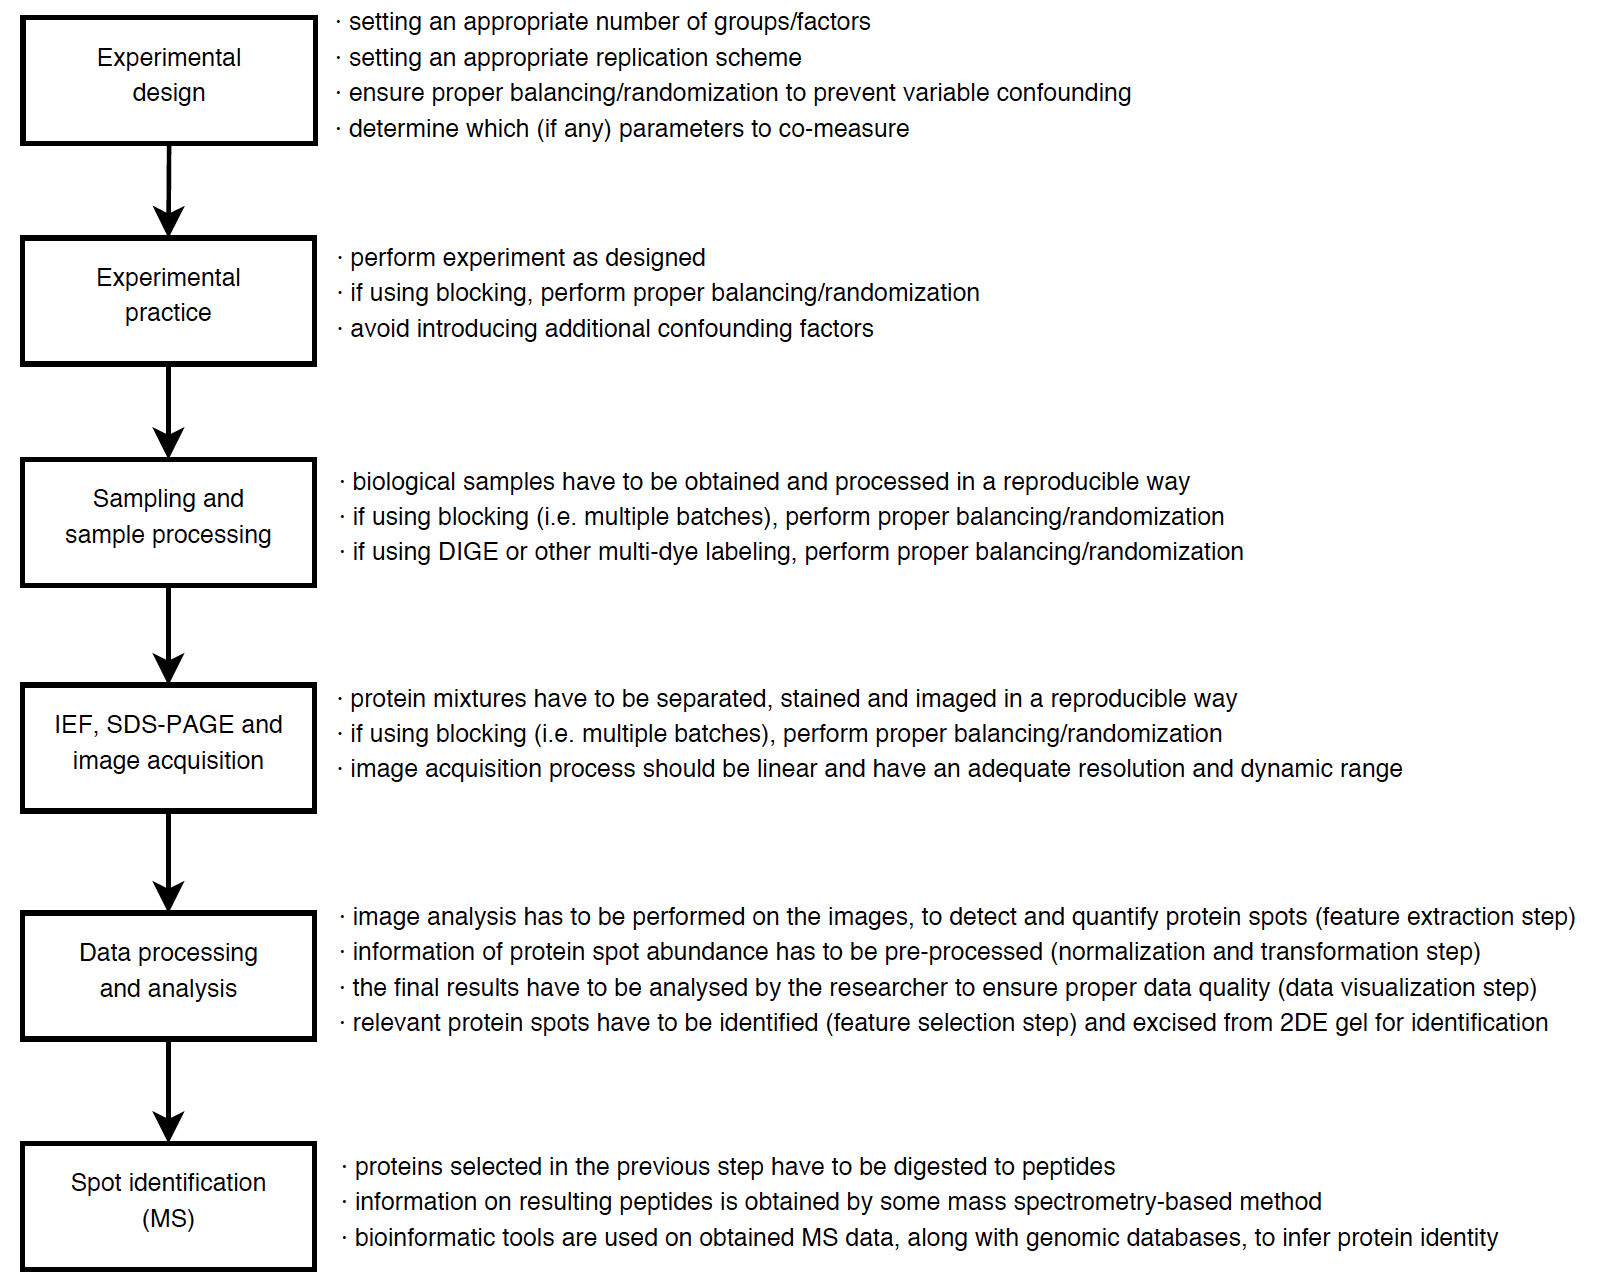
\includegraphics[width=\textwidth]{figures/gel-based.png}
\caption[High level overview of a typical gel based proteomics workflow.]{High level overview of a typical gel based proteomics workflow \cite{SIL2014}.
\label{fig:gelflow}}
\end{figure}

There are different protocols for gel-based experiments to try to overcome the different limitations of this technique (i.e. low resolution, low dynamic range and low reproducibility), and Differential Imaging Gel Electrophoresis (DIGE), has become one of the best alternatives. The main difference between DIGE and other protocols is that control and case samples are tagged with different fluorescent dyes, which facilitates spot detection and its posterior quantification \cite{PAN2008}.

In most of the protocols, each of the gels can have other variables associated with them, for instance the tissue that it belongs to, information about the donor (e.g. sex, age, weight) and data about the hypothesis (e.g. healthy/infected). The relevance of a spot in the context of the study hypothesis and considering all the mentioned variables, is used to filter the required protein identification experiments, and ultimately reduce time and costs to prove/disprove the hypothesis. It is in this step where statistical and visualisation techniques are of great assistance to the researcher \cite{SIL2014}.

The problem is that common visualisation techniques (e.g. box plots, scatter plots) are usually not sufficient, because the number of variables (spots) to include is too high (in the order of hundreds), and therefore multivariable techniques that combine statistical methods and visualisation tools are required at this stage.

Principal Components Analysis (PCA) has become the preferred technique in 2D PAGE, because it offers a good and unbiased view of a dataset along the subspace where most variation occurs. PCA looks for a 2D or 3D representation of the data where the axes are the principal components PC (hence its name) that most effectively contribute to determine the variance of the data. A PC is not a single variable but rather a projection of the combination of several, and the result of a PCA gives the contribution of each of the variables to each PC.

Figure \ref{fig:PCA}, which was originally published in \cite{SIL2014}, serves as an example of the visualisation of the results of a PCA on a data set in which two treatments (``A'' and ``B'') were compared with biological samples being taken at three time-points: 0h, 6h and 48h; colour-coded as light grey, dark grey and black respectively. There is a clear division of two groups. In a 2D PAGE experiment, it is common to select the spots to analyse further by studying the variable contribution on each PC.

\begin{figure}  
\centering
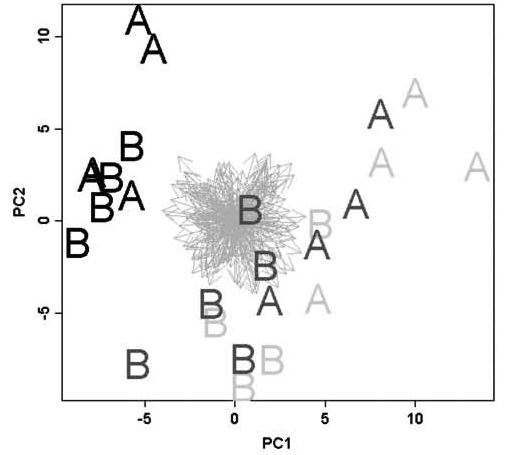
\includegraphics[width=4in]{figures/PCA.png}
\caption[Example of a PCA result plot.]{A biplot displaying PCA results. Figure taken from \cite{SIL2014}. 
\label{fig:PCA}}
\end{figure}

PCA uses the Euclidean distance when calculating the projections of the variable contributions on each PC. This strategy has shown a good balance of outcome/performance for multidimensional data, however when the number of dimensions is very high it can be misleading, and then other techniques are necessary, e.g. Independent Component Analysis (ICA), Partial Least Squares (PLS), Metrical multi-Dimensional Scaling (MDS), Non-Metrical multi-Dimensional Scaling (NMDS), clustering methods and Self-Organised Maps (SOM). A discussion about the use of these methods in 2D PAGE analysis can be found in \cite{SIL2014}.



\subsubsection{Mass Spectrometry Techniques}
Proteomics based on mass spectrometry focused on identifying, quantifying and characterising as many proteins as possible in a single experiment . Probably the tipping point for the usage of MS techniques was the development of tandem mass spectrometry (also known as MS/MS) because it allows the identification of a large number of proteins using high throughput techniques \cite{PAN2008}.

An MS experiment is commonly the next step following a protein separation process. In the case of 2D PAGE, the spots are cut out of the gel, and the proteins are digested into shorter peptides by an enzyme (e.g. trypsin) and then separated in order to reduce the sample complexity and to get better performance out of the mass spectrometer.

The workflow to analyse MS/MS results is described in figure \ref{fig:ms_workflow}. The input is the raw data generated by the mass spectrometer, whose format is usually native to the machine, and therefore the first step is to convert the files into more standard formats \cite{DEU2008}. 

The mass spectra data of each peptide is used to try to identify the protein which usually involves searching for similar mass spectra of known (or hypothetical) peptides; followed by a validation step, and then the inference of the target protein is calculated.

The subsequent stages in the workflow are dependant on the nature of the experiment (e.g. requires quantification because it is a comparison of control v.s. sample) or the setup of the laboratory (e.g. it uses a Laboratory Information Management System LIMS, or not). \cite{DEU2008} includes a more complete description of this workflow and the most well-known software tools associated with each step.

\begin{figure}  
\centering
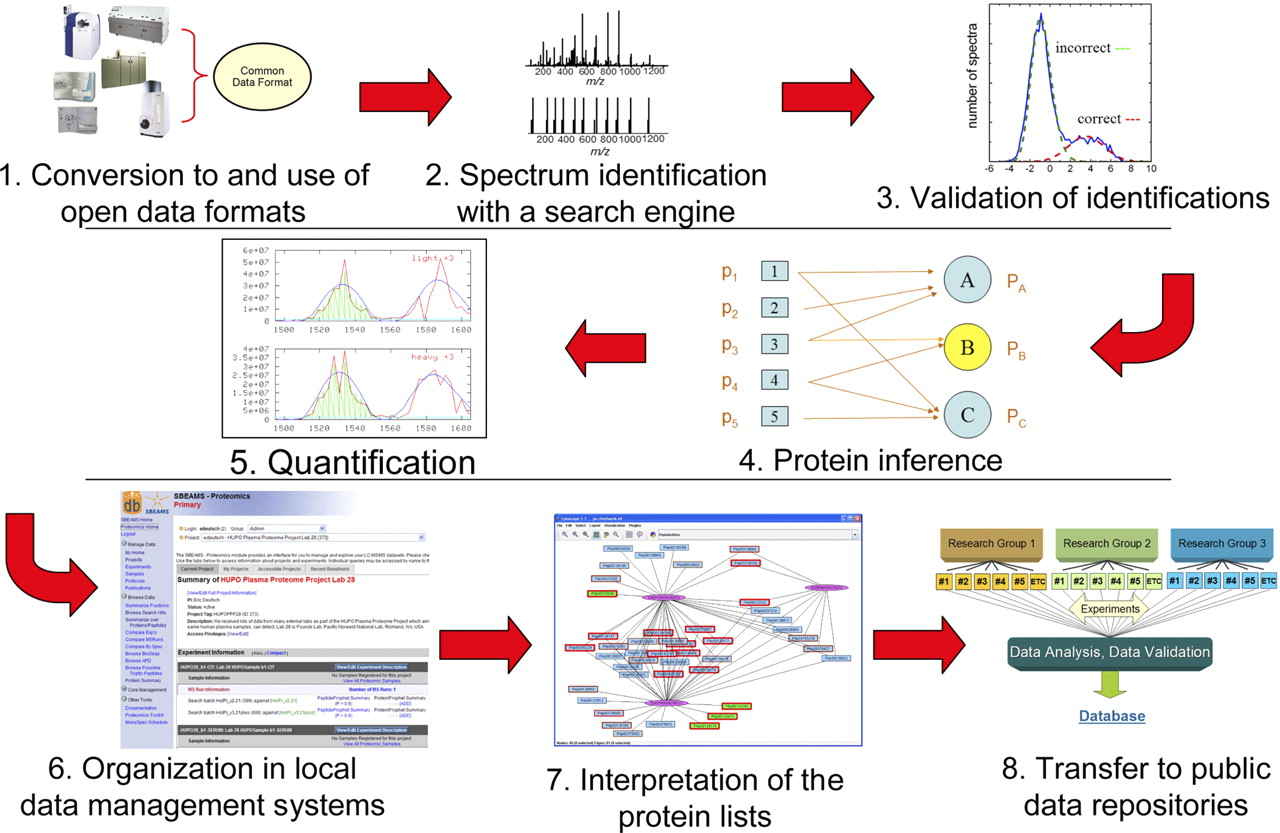
\includegraphics[width=6in]{figures/ms_workflow.png}
\caption[Tandem mass spectrometry workflow.]{Tandem mass spectrometry workflow \cite{DEU2008}.
\label{fig:ms_workflow}}
\end{figure}


A classification of the most frequent tasks based on the described workflow have been included in \cite{PER2014} in order to describe the contributions of different open source libraries in MS experiments. Below we describe the two software tools mentioned there that include several visualisation techniques to aid in the different stages of the MS workflow. An extended list of visualisation tools in MS/MS based proteomics can be found in section 5 of \cite{JAC2010}.

\paragraph{PRIDE Inspector}
The PRoteomics IDEntifications database, PRIDE, is a centralised repository where proteomics data is stored and shared. In order to submit data into PRIDE, a series of standards have to be followed, which ensures the high quality of the data. These types of resources have been used more often, in part because some journals require that for an article to be published, its data should be stored in a public repository that follows community standards.

PRIDE Converter (\url{https://code.google.com/p/pride-converter/}) is a tool that provides support during the process of submitting new data to PRIDE. The same team developed PRIDE Inspector following the success of the converter, and motivated by the fact that inspection and validation of reported results are of great importance during the review process \cite{WAN2012}.

\begin{figure}  
\centering
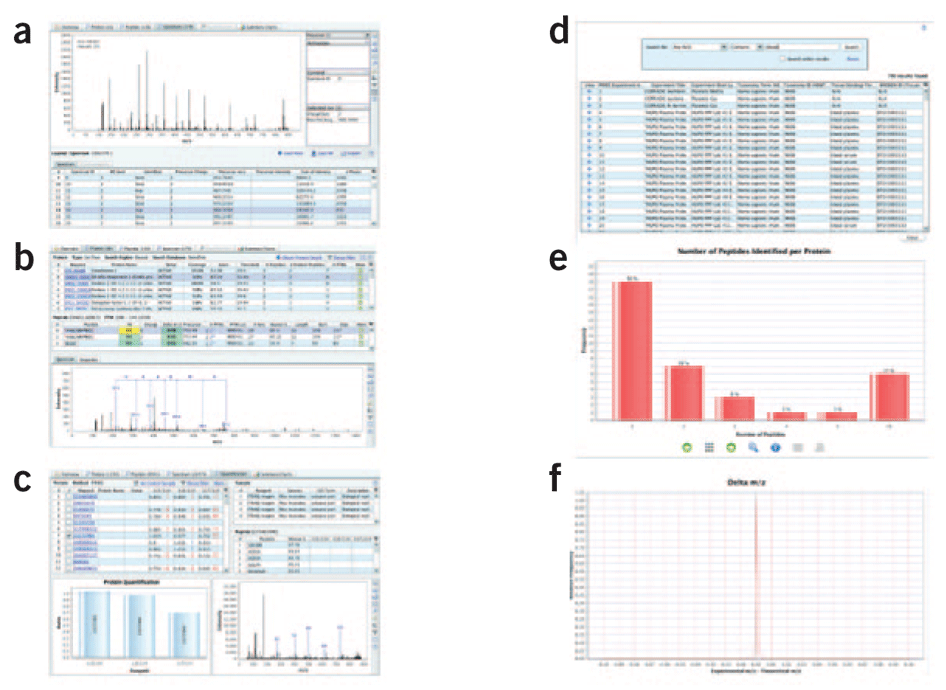
\includegraphics[width=\textwidth]{figures/prideinspector.png}
\caption[Snapshots of the PRIDE inspector toolset.]{Snapshots of the PRIDE inspector toolset: (a) Section of the spectrum view tab. (b) Protein view tab, including the spectrum viewer showing MS/MS fragment ion annotations (only b ion annotations are shown). (c) Quantification view. (d) 'Search PRIDE' panel. (e) Number of peptides identified per protein chart. (f) 'Delta m/z' chart.
\label{fig:pride}}
\end{figure}

Figure \ref{fig:pride} is a group of some of the views of the PRIDE Inspector application. The user can load their own data or explore the public data from PRIDE using the search view (d). The proteins of the data set are listed (b) including their peptides, post-translational modifications PTMs and corresponding spectra. The spectrum viewer (a) includes automatic annotations based on submitted fragmentations. Some aggregate charts (e) and (f) are also available to explore the information for each protein, and if the experiment includes quantification data, the view in (e) is enabled and the data can then be used to create comparative charts.

PRIDE Inspector was developed with modularity in mind, and as a consequence, libraries packaging some of the functionalities can be obtained independently. The visualisation routines are accessible from a library called mzGraph that can be reused in other projects.

\paragraph{Rover}
The open source Java application called Rover, focuses on quantitative proteomics data. It generates visualisations of this data that help the user in the process of selecting and validating algorithm-suggested regulated proteins in the context of an experiment \cite{PER2014}.

Quantitive proteomics datasets are composed of two parts in Rover: peptide identifications and quantitative data. Rover includes a wizard-like menu that facilitates the input of these files. It also includes several parsers for some of the most frequently used formats of this type of data.

\begin{figure}  
\centering
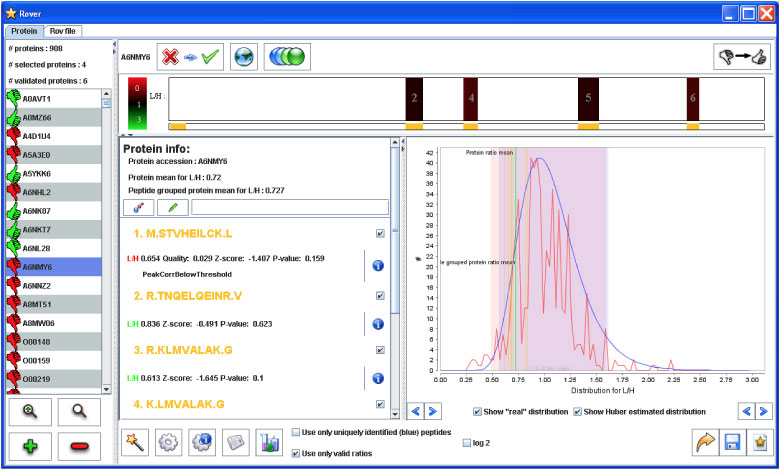
\includegraphics[width=\textwidth]{figures/rover.png}
\caption[The main Rover interface.]{The main Rover interface \cite{COL2010}.
\label{fig:rover}}
\end{figure}

Once the data has been successfully loaded into Rover, a high level view of it is presented to the user so they can choose and validate the set of proteins proteins automatically selected based in their peptide ratio. 

Figure \ref{fig:rover} shows a snapshot of the main interface of Rover. It displays protein and peptide information as follows: on the left side there is a panel displaying all the proteins that are part of the experiments; glyphs are used to indicate if the protein is selected (thumbs up) or not (thumbs down), and it is colour coded, the protein is green if validated or red if not validated. The top of the screen is the protein bar, where the peptides are drawn proportionally over a rectangle that represents the whole protein. The centre of the window is then divided again: the left side offers general information on the selected proteins and the right side displays the ratio distribution graph, where the selected protein and its ratios are shown in comparison to the reference set, using either the intrinsic distribution of the data or transforming the data to use the Huber distribution, which can provide a new perspective on the analysed data \cite{COL2010}.

All data generated with Rover can be exported for subsequent analysis.

\subsubsection{Microarrays}
Although Microarray techniques are considered by some to be out of the proteomics field because they deal with transcription data more often than with proteins themselves, this technology offers a high throughput solution to study the expression levels of genes on a particular sample. Although the level of expression of a gene is not sufficient to evaluate the number of proteins produced, it is considered to be a good indication.

There have been advances in microarray techniques that use proteins in order to complement MS studies \cite{PRA2014}. Because of their high usage we will focus on visualisation tools used in the analysis of DNA/RNA microarrays. In particular, we will describe two suites that serve to exemplify the most common scenarios where visualisation techniques are applied to microarray data. This, however, is just a small sample of all the tools that are used to analyse this type of data.

\paragraph{Bioconductor}
Bioconductor is a library for the programming language R, that aims to provide support for general research in computational biology. They have orientated their efforts towards the statistical analysis of microarray experimental data, covering many of the usual tasks required: preprocessing, quality control, normalisation and downstream inference of biological and clinical questions \cite{GEN2004}.

The development of Bioconductor has been inspired by the achievements of other software that follow the principles of the Free Software Foundation. The authors consider that the adoption of these principles for the computational biology and bioinformatics fields is key to improving research in terms of transparency (i.e. exposure of the entire process), reproducibility and efficiency of development.

R is a programming language recognised for its numerical and statistical capabilities, which can be easily connected to many types of visualisation graphs. R can be used for rapid prototyping and quick exploration of data. It supports multiple network and parallel computing protocols, as well as access to different database systems \cite{IHA1996}. These are some of the factors that attracted the Bioconductor community when they were choosing which language to use to implement their goals \cite{GEN2004}.

The Bioconductor project has invested much of its time into the creation of the project infrastructure, for example, by defining protocols for submission of new packages and their documentation; interfaces to the existing packages; documentation for both user and developer; exposure to the documentation from within the system; guidelines on how to use their source code repository; definition of good practices when developing a Bioconductor packages, etc.

Thanks to these efforts, Bioconductor now has a strong community of users with more than 3000 subscribers to their forum and over one million visitors to their website, on which it is possible to find over 800 software packages (release 2.14). Their publication \cite{GEN2004} has more than 6000 citations and many of the packages developed for Bioconductor have also been published in peer-reviewed journals \cite{BIO2014}.


\begin{figure}  
\centering
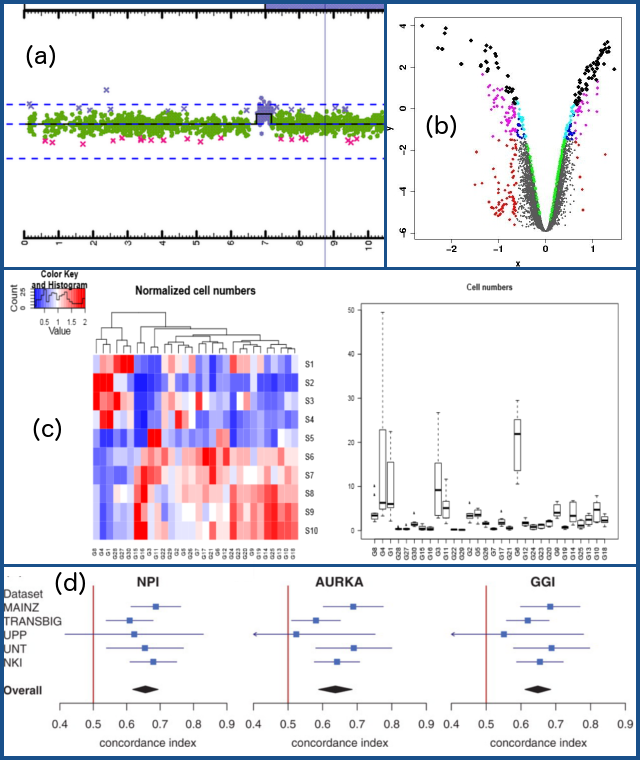
\includegraphics[width=\textwidth]{figures/bioconductor.png}
\caption[Visualisations created with Bioconductor's packages.]{Visualisations created with Bioconductor's packages, taken from their respective web sites: (a) aroma (\url{http://www.aroma-project.org/screenshots/}). (b) arrayQuality (\url{http://arrays.ucsf.edu/}). (c) flowCyBar (\url{http://www.ufz.de/index.php?de=32737}). (d) survcomp (\url{http://www.pmgenomics.ca/bhklab/software/survcomp}).
\label{fig:bioconductor}}
\end{figure}

In terms of visualisation, the Bioconductor repository had 218 packages listed with the visualisation tag by January 2015 (\url{http://www.bioconductor.org/packages/release/BiocViews.html#___Visualisation}). Figure \ref{fig:bioconductor} is a random selection of snapshots from several packages found on that list. This includes: (a) Aroma (\url{http://www.aroma-project.org/screenshots/}), which provides a view similar to that of genome browsers in order to display copy-number amplification in a chromosome; (b) a diagnostic plot generated by arrayQuality (\url{http://arrays.ucsf.edu/}); (c) a clustered heat map and box plot, resulting from the analysis of cell abundance changes in subcommunities deployed by using flowCyBar (\url{http://www.ufz.de/index.php?de=32737}); and (d), part of the case study used to describe survcomp (\url{http://www.pmgenomics.ca/bhklab/software/survcomp}), a package created to compare the performance of survival/risk prediction models. 


\paragraph{Chipster}
Chipster is a software suite that includes many of the most frequently used software tools for the analysis and visualisation of microarray data and other high throughput experiments. It has a client-server architecture where the client is a graphical oriented interface that allows not only the display of, but also interaction with visualisations. The server on the other hand is oriented to the execution and administration of the tools that a particular Chipster installation offers.

Chipster extensively supports the Bioconductor package, allowing the editing of scripts to include functionalities from the R package. Other tools can also be imported to Chipster, however only those written in Bioconductor can be edited through Chipster.

Chipster is an exploratory tool where different tools and visualisations can be used at any time, guided by the user's will. Moreover the execution history is saved as a workflow, and therefore it is easy to re-execute with different data or tune the different tools' parameters. The workflow files can also be saved and shared.

There are more than 25 visualisations included in Chipster. Those generated for the client software can be manipulated by the user, and they also serve as a way to interact with, select and filter the data. The visualisation generated by Bioconductor and other imported tools are treated as static images and basic zooming and panning is supported. The interactive visualisations include scatter plots, volcano plots, venn diagrams, heat maps, self organised maps, among others; and can be used for different stages of a microarray experiment, e.g. normalisation, quality control, filtering, statistical testing, clustering, annotation, etc. \cite{KAL2011}. 


\subsubsection{Protein Annotations}
There are several projects that provide visualisations similar to those offered by genome browsers, but in where reference and features are protein data. The challenges for these types of applications can be slightly different to their genome browser analogues. For example, one of the biggest challenges of the latter technology is how to deal with the length of a genome, and therefore those applications have developed strategies for smart panning navigation, only loading by-request and offering several graphic interface gestures to navigate through a chromosome as seamlessly as possible. For protein browsers the length is not a major concern, as proteins are usually less than a thousand amino-acids long, and at present most computer screens use resolutions higher than 1024x768, so the inclusion of a representation of the whole protein on the screen should be relatively simple.

On the other hand, the number of sources of protein data can be quite large, and therefore strategies are required to deal with the vertical growth of the visualisation. For example, grouping annotations on the same track, or some kind of vertical panning/scrolling. Below we briefly describe some of the most recognised protein annotation browsers, and in section \ref{section:dasty} we discuss Dasty3, a protein feature viewer to which we have contributed during this PhD.

\paragraph{PFAM} 

\begin{figure}[ht]
\centering
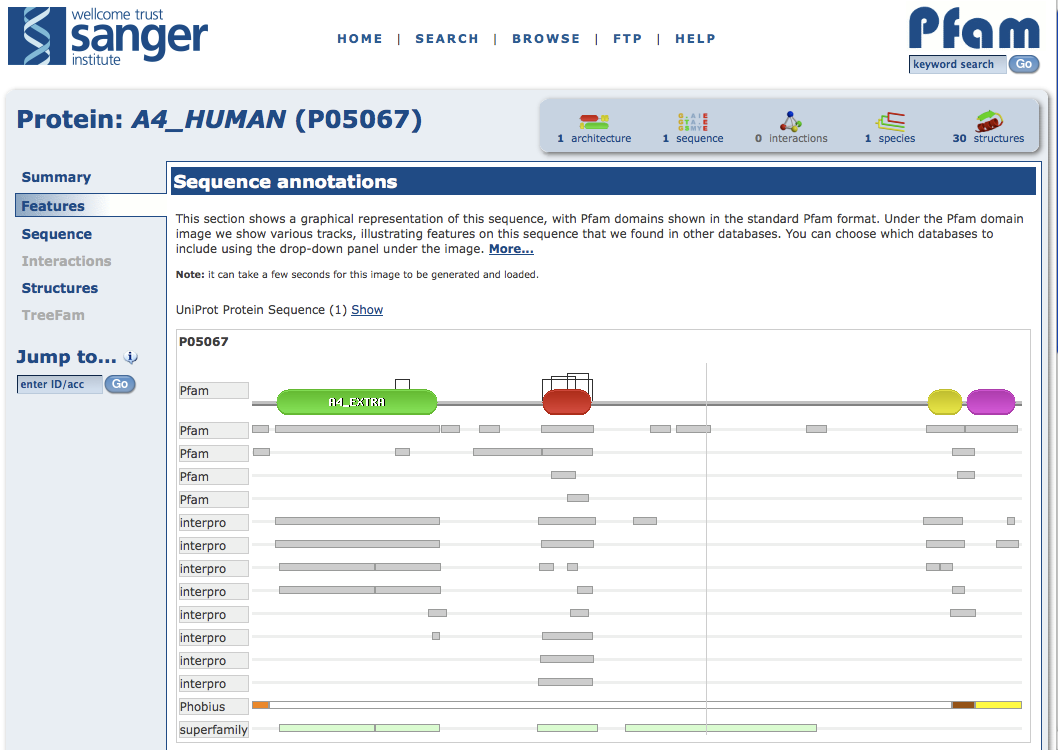
\includegraphics[width=6in]{figures/pfam.png} 
\caption[PFAM Snapshot] {\emph{PFAM}: Web widget, which places special emphasis on the visualisation of the annotations of protein domains} \label{fig: pfam}
\end{figure}

The Protein Family Database (PFAM) project's main goal is to provide information for protein families and domains. The database is divided in two subsets: PFAM-A contains curated information and PFAM-B is an automatically generated database \cite{FIN2008}. 

The PFAM website provides several ways to access this data, one of them being the feature viewer, where, besides PFAM's own annotations, it allows users to get information from other sources and to put it in the same context. Figure \ref{fig: pfam} shows the result of a query in the PFAM feature client. The first track contains all the annotations about families and domains that the PFAM database provides. The next set of tracks are the rest of the annotation sources that PFAM provides. Finally all the features of external data sources that the user has selected for that query are shown \cite{FIN2008}.

\paragraph{InterPro} 
The InterPro database is a public resource used to classify sequences into protein families, which are annotated, and subsequently used to infer features of non-annotated proteins. InterPro combines the data from different databases, and has grown from four sources in 1999 to eleven in 2014. The combined resource provides information about protein families, domains and functional sites.

At the core of InterPro are protein signatures, which are representations of groups of protein sequences based on similarity. These are annotated with a name, a descriptive abstract and gene ontology (GO) terms. Functional features of a signature can be used to describe a protein by identifying the existing signature in the target protein. This approach has predicted the function of almost fifty million individual proteins \cite{MIT2014}

\begin{figure}[ht]
\centering
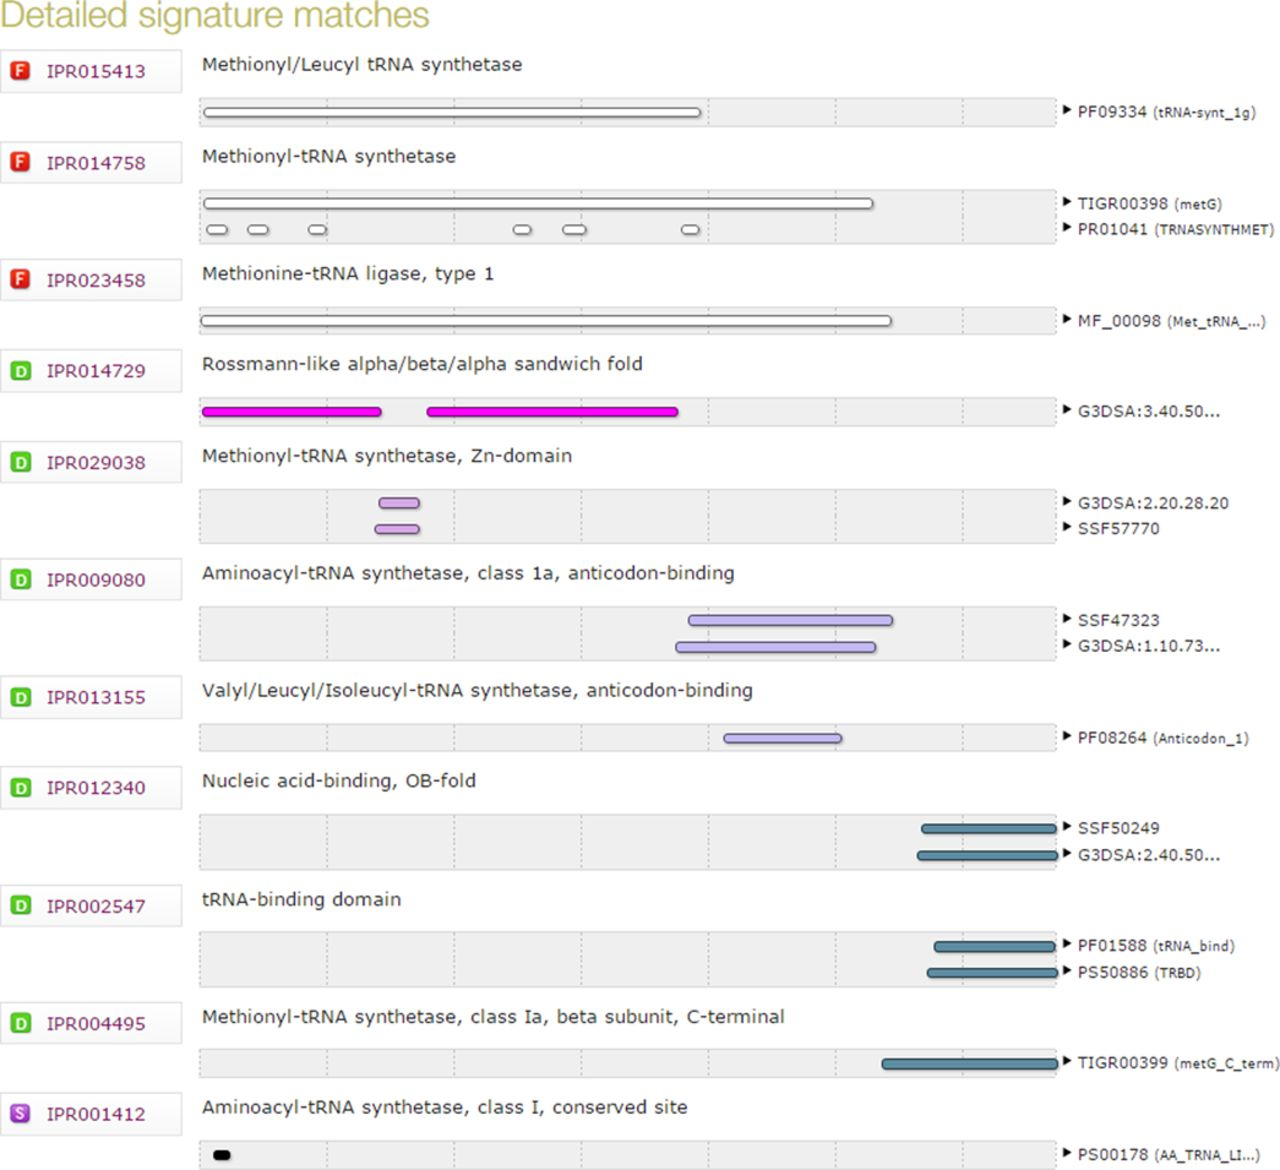
\includegraphics[width=6in]{figures/interpro.jpg} 
\caption[Interprot Snapshot] {Detailed InterPro member database match data for UniProtKB entry Q3JCG5} \label{fig: interior}
\end{figure}

Figure \ref{fig: interior} is a snapshot from the InterPro website, displaying sixteen individual signatures from seven sources, that have been grouped into eleven entries.
It uses a similar visual approach to other protein annotation viewers, in which features are located proportionally to the reference, but in this case the reference is not another track on top, but instead is a box on which the annotations are included. In this way the reference is always visible, no matter how many entries are on display or how far have the user has scrolled. However, this view takes more space and as a consequence, less tracks can be displayed simultaneously. 

\subsection{Protein Interactions}
\label{sec:ppi}
Interaction between proteins is one of the most important mechanisms in the execution of cellular functions. The study of these interactions has provided insight into the functioning of an organism's processes.

The number of reported Protein-Protein Interaction (PPI) networks has grown considerably, partly due to advances in high-throughput experimentation and partly due to the new predictions that result from these empirical data. For example, as of January 2015, \emph{Homo sapiens} had over 300000 Protein-Protein interactions (PPI) registered in the Interologous Interaction Database \cite{NIU2010}, which is only one of the many public resources where protein interactions can be accessed for different species. 

Data repositories for PPI data can be classified into three groups: (i) Primary interaction databases, where curated experimental results are deposited, for example: IntAct \cite{KER2012}, MINT \cite{LIC2012}, BioGRID \cite{STA2006}, DIP \cite{SAL2004} and HIPPIE \cite{SCH2012}; (ii) computationally predicted databases, for example, DIMA \cite{LUO2011}, PIPs \cite{MCD2009}, PrePPI \cite{ZHA2012} and PRISM \cite{OGM2005}; and (iii) databases integrating both types of data, for instance, GeneMANIA \cite{WAR2010}, FunCoup \cite{SCH2014}, I2D \cite{NIU2010} and STRING \cite{SZK2014}.

The volume of data that PPI repositories have reached has made their analysis and understanding a challenge that can be enriched by the use of visualisation techniques. PPI networks have been found to follow a behaviour that in graph theory is referred to as \emph{scale-free}, which has a few highly connected nodes and many nodes with few interactors. This feature allows the user to predefine visualisation strategies to highlight certain characteristics.

The list below was identified in \cite{AGA2013} as the main requirements for the visualisation of protein interaction networks:
\begin{itemize}
\setlength\itemsep{-0.3em}
        \item Clear rendering of network structure and sub-structures, such as dense regions or linear chains;
        \item Fast rendering of huge networks;
        \item Easy network querying through focus and zoom;
        \item Compatibility with the heterogeneous data formats used for PIN representation;
        \item Interoperability with PPI databases, allowing the automatic querying of single or multiple databases using existing middleware;
        \item Integration of heterogeneous data sources, e.g. functional information about proteins extracted from biological ontologies.
\end{itemize}

There are several tools that allow the exploration of PPI data, providing different methods to visualize protein network interactions. \cite{AGA2013} evaluates some of them by considering the requirements above. Other surveys can be found in the literature where comparisons and descriptions of several PPI tools are included \cite{SUD2007, PAV2008, GEH2010}. Below, we describe some of these and in section \ref{section:pinv} we explore in detail PINV, the web based PPI visualisation tool we developed. 

\subsubsection{STRING}
STRING is a repository for PPI data that includes both primary and computationally predicted interactions. It differentiates itself from other resources such as those mentioned above in three ways: coverage (more than 2000 organisms), the inclusion of text mining data, and the metadata linked to the interactions (e.g. protein domains and structures) \cite{FRA2013}.

STRING includes a viewer developed in Adobe Flash that allows the direct manipulation of the graph based on mouse interaction. The network to be displayed in the viewer is the result of a user query of either one or multiple proteins. However it can also be invoked by a call to one of the resources that are cross-linked to STRING.

\begin{figure}  
\centering
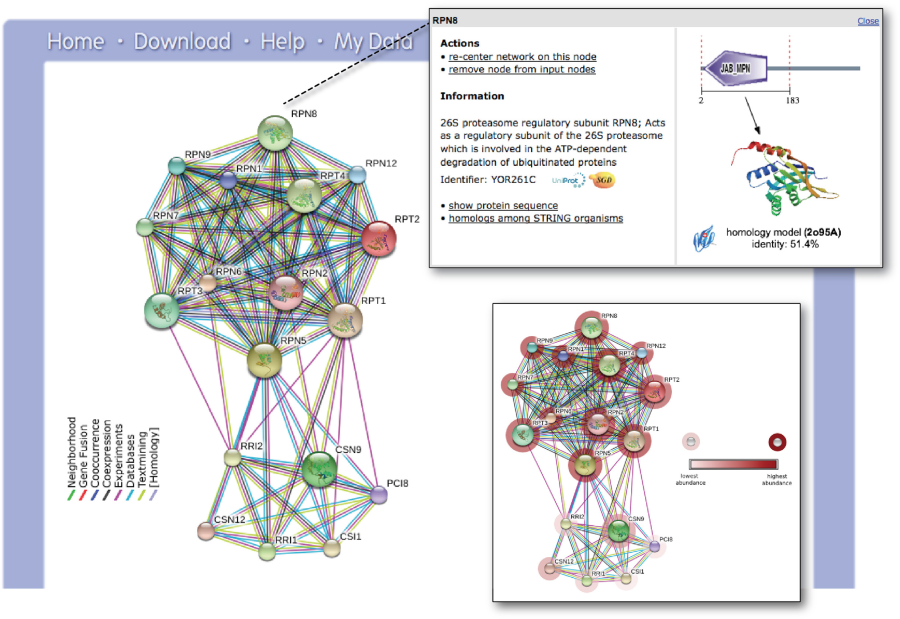
\includegraphics[width=\textwidth]{figures/string.png}
\caption[STRING Snapshot.]{Combined screenshots from the STRING website
\label{fig:string}}
\end{figure}

Each protein node includes a preview of the 3D structure (if available). When the user clicks on the node, a popup window opens with extra information about that protein, including links to external resources such as PDB or UniProt. The interactions between the proteins are represented by multiple lines representing the different sources of evidence; clicking on an interaction opens another popup window with more details on the evidence data. See figure \ref{fig:string} for an example of the viewer including a pop-up window for protein details.

One of the most recent developments in STRING is the creation of a Bioconductor package that can access STRING information directly from the R programming language in order to allow automation of the data collection from this resource. This feature is an addition to previously released  data access services: REST and the ability to download version-based compressed files of all the interactions in STRING \cite{SZK2014}.

\subsubsection{Cytoscape}
Cytoscape is ``\emph{a free software package for visualizing, modeling and analyzing molecular and genetic interaction networks}'' \cite{CLI2007}. It is arguably the most used tool to create visualisations of biological networks, and has a general purpose architecture that provides the environment to model biomolecular interaction networks. We consider that besides being a useful software that reaches the expectations of a network visualiser, there are two major factors for its success: Cytoscape has a well designed architecture with robust support for plugins (called apps since Cytoscape 3.0) and it follows an open source philosophy.

The success of the project is apparent in its growth: In the welcome letter (\url{http://cytoscape.org/cy3_welcome_letter_v12.pdf}) of the project to their users dated on November 7, 2014 they report having an average of 12000 downloads of the application per month and noted that it has been opened 2000 times per day worldwide. In addition, Cytoscape now has over 200 plugins available in its App Store, a clear example of its collaborative environment, where scientists/developers can contribute to the network analysis toolset by adding new plugins.

The core of Cytoscape is their network graph, which uses the previously mentioned node-link technique, where the nodes can be any type of biological entity (e.g. genes, proteins, organisms) and the links are the pair-wise interactions \cite{SHA2003}. It is important to note that the decision to use a generic representation for nodes and links is a factor that has attracted users from the different domains of the biological sciences. This is as opposed to exclusively link the generic representation to proteins or genes for example, as has been implemented by similar projects.

The network graph can be manipulated by the user selecting where to locate a node, however this task needs to be automated in order to save time and be able to deal with many nodes. Cytoscape provides many automatic layouts on its basic installation and there are more options available as plugins.

The network can be enriched by two means: attributes and annotation. Attributes are name-value pairs that can be associated with either a node or a link. The concept of an annotation in Cytoscape is similar to that of the attribute, because it is also an association to a network entity, but annotations require the use of ontologies (e.g. gene ontology) in order to follow a hierarchical structure for filtering and manipulation.
This information can be added by different means: (i) manually included by the user (i.e. by using the spreadsheet interface), (ii) calculated by the tool or one of its plugins (e.g. network attributes such as the degree of a node), (iii) extracted from an on-line resource (e.g. getting the GO terms from UniProt), (iv) imported from a local file (e.g. expression values per protein) \cite{SAI2012}.

\begin{figure}  [t]
\centering
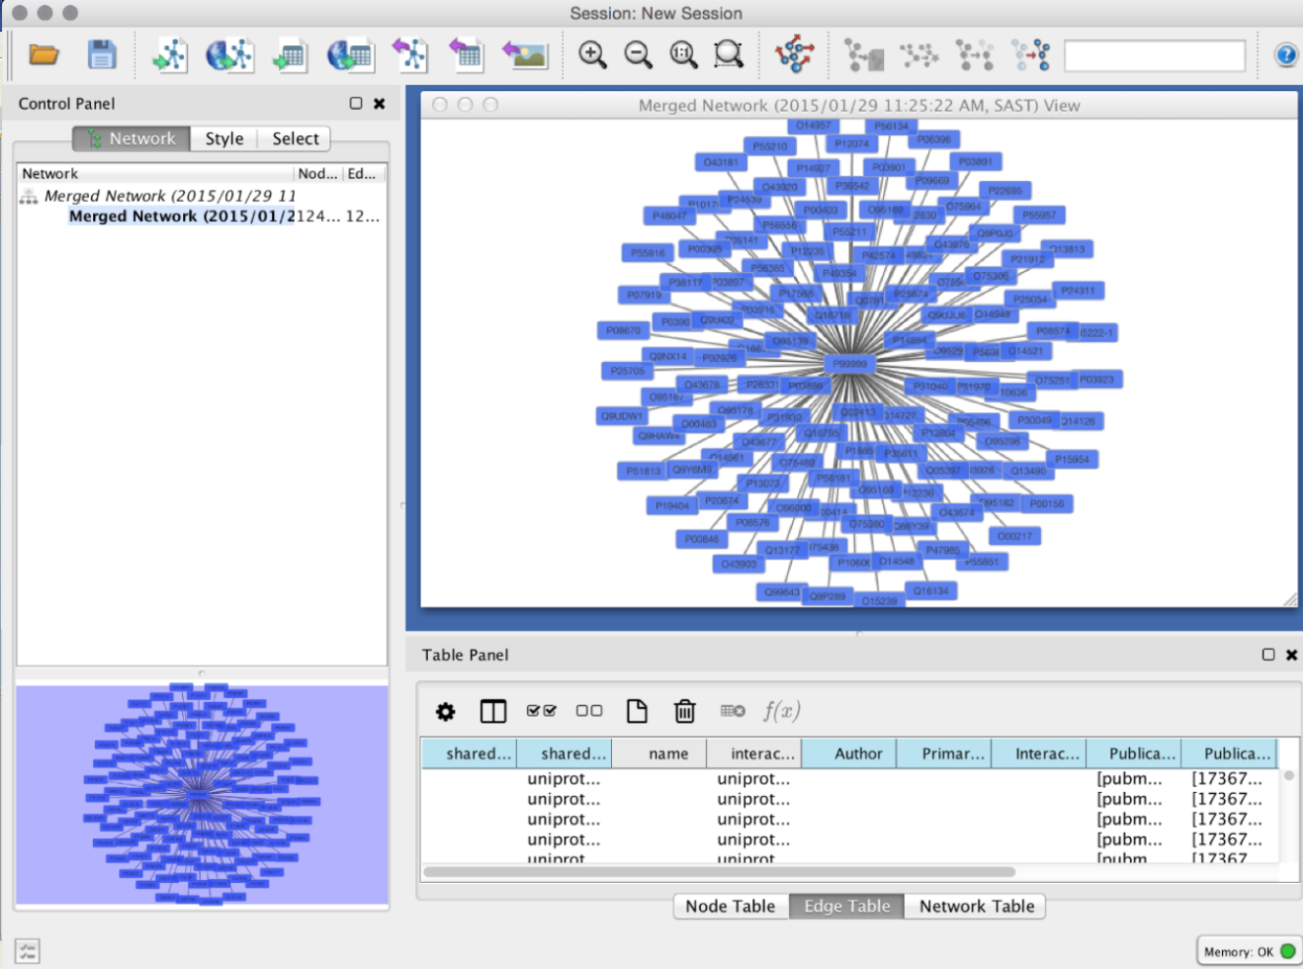
\includegraphics[width=\textwidth]{figures/cytoscape.png}
\caption[Cytoscape Snapshot.]{The Cytoscape Desktop.
\label{fig:cytoscape}}
\end{figure}

Figure \ref{fig:cytoscape} shows the graphic interface of Cytoscape 3.2.0 running on a Mac OS X. Quick access to the most frequently used tools have been grouped in the top bar. The left panel provides a hierarchical structure to navigate though the current networks and includes a zoomed out view of the graph; the main panel is the Cytoscape canvas where the network graph is on display, and at the bottom-right is the spreadsheet interface that allows the user to browse the attributes.

The most basic uses for attributes and annotations are to filter the network by selecting only the nodes with an attribute of interest. They can also be used to map the information onto the graphic by altering colour, shape and size of the nodes and links, according to the value of a specific attribute, allowing the user to visualise several types of data within a single view. However the use of this metadata can also be extensively used by the plugin's developers in many other complex scenarios.

Besides the growth of the application due to the development of new plugins, the core application is continually updated by adding new features and fixing bugs. For example, two major features were included when version 2.8 of Cytoscape was released: the possibility of using an image to represent the node, and the support for equations on the spreadsheet view of the network. Although both functionalities were previously available via Cytoscape's API, their inclusion in the main application facilitates their use by non-programmers \cite{SMO2011}.

A protocol describing a common workflow in Cytoscape was published in \cite{CLI2007}. In it, a classification of the most common tasks is included and used to structure the document. The five tasks identified were: 
\begin{itemize}
\setlength\itemsep{-0.3em}
        \item \emph{Obtain network data}: The user has several options to do this, including loading local files in one of the multiple supported formats, importing data from an on-line resource such as MINT or STRING or invoking text-mining plugins that analyse literature resources such as PubMED to infer reported interactions of genes or proteins of interest.
        \item \emph{Explore network and generate layout}: As mentioned before, several automatic network layouts are included in Cytoscape.
        \item \emph{Annotate with attribute and expression data}: The results of an expression experiment can be mapped to an existing network by, for instance, colouring the nodes in a scale from green to red, in order to easily identify over and under expressed genes in the graphic.
        \item \emph{Analyse network features}: The entities included in the network can have associated functional classes, and the discovery of clusters or hubs can be relevant to the biological understanding of the system.
        \item \emph{Detect enriched functions}: The same information can also be used to infer functions for other entities that were not well annotated.
\end{itemize}

Given the growing number of apps, the Cytoscape team developed the App Store, which was released together with version 3.0 of Cytoscape in 2013. This service attempts to provide a showcase for developers to display their contributions to the Cytoscape community, and for users to find the right tool to complement their research. App authors can include screenshots, descriptions, links and other metadata in order to highlight the features of the app and facilitate its use. App store users can navigate though the categories, search by their attributes, or select one from the list of featured apps. Besides providing information, the App Store also allows apps to be installed and upgraded with a single click \cite{LOT2013}. 

\subsubsection{Web based PPI tools}
As stated in \cite{GEH2010} ``\emph{there is a trend toward web-based applications, often coupled tightly to underlying databases}''. STRING (described above) is a clear example of this tendency, where an effort to integrate PPI information in a centralised resource is combined with a tool that allows the search, exploration and visualisation of such resources. Most interactive online visualisation tools follow this path, only allowing the view of networks that are preloaded, meaning that the user cannot view a network he/she has generated.

The online version of Graphle \cite{HUT2009} is limited to graphs generated by bioPIXIE in yeast, MEFIT in \emph{E. coli}, or HEFalMp for human data. STITCH \cite{KUH2008}, a project for chemical-protein interactions, integrates interaction information from various sources in addition to in-house predictions. Both STRING and STITCH use the same library to display their data. However, the network visualized in both databases is barely customizable. The public implementation of VisANT \cite{HU2013}, a workbench for the integrative analysis of biological networks, is based on the Predictome database. Although these tools are available on the web, they require third party software (e.g. Adobe Flash, Java Virtual Machine) and therefore their accessibility is more limited than native web applications (i.e. developed using recent web standards). 

Another alternative is Cytoscape Web \cite{LOP2010}. Its introductory tutorial (\url{http://cytoscapeweb.cytoscape.org/tutorial}) requires users to code in JavaScript indicating that this tool is mainly intended for developers to display networks on the web, and not for the scientist who has a network to visualize. Cytoscape Web also uses Adobe Flash for the generation of the graphics. A more recent development is Cytoscape.js (\url{http://cytoscape.github.io/cytoscape.js/}), which uses the HTML5 component called canvas, and therefore its only dependency is a modern web browser. The principles behind this project is to offer a modern web toolset to display interactions. Similarly to its predecessor, Cytoscape.js is a library for programmers, and is intended to be a complement to the Cytoscape Desktop.

A native web application that supports the visualisation of networks and is intended for non-programmer users is Pclust. Its objective however is not the visualisation of PPI networks. Pclust is a tool that assists in the inference of functions of new proteins from their homologs, using a technique known as all-against-all pairwise similarity. The network is built by looking for similar functionality between proteins. The set of proteins can be either entered by the user or detected by executing a BLAST (Basic Local Alignment Search Tool) against the non-redundant (NR) database. The resulting network is then enriched with related literature through the Seq2Red server (\url{http://prodata.swmed.edu/seq2ref/}). The visualised network creates clusters of proteins with similar functionalities. Proteins with references are highlighted, which helps to solve ambiguities in the deduced functions \cite{Li2013}.


\subsection{Discussion} \label{sec:intro-discusion}
The projects described above gave us a clear insight into the influence that visualisation techniques have on molecular biology research. We have only mentioned a few cases in the field of genomics, proteomics and protein-protein interactions networks, but the visualisation techniques have been applied to many other fields such as metabolic pathways (and system biology in general), population genetics, metagenomics, etc.

It is important to note that each scenario required a different visualisation technique, from simple two dimensional plots used to display complex statistics (e.g PCA), to highly detailed tools that combine more than one visualisation technique, for example, genome browsers.

Genome browsers have evolved from simple displays of genes and transcripts to become visual integration tools of biological data. Tracks can be preprocessed using many combinations of statistics and data analysis, and its visual representation can vary from simple boxes to histograms, heat maps, and many other charts. This is not unique to genome browsers and the exploration of biological data have required the use of the whole range of visualisation strategies in an attempt to illustrate specific biological cases, and ultimately to contribute to our understanding of life.

One of the most appropriate ways to evaluate the success of software applications is through the number of users, developers and collaborators involved in the project. A large community can detect errors and improvements faster, and therefore act quicker, which ultimately makes the software improve faster. This, in turn, means, more users are attracted to build an even bigger community, and to restart this positive cycle.

A common denominator in successful visualisation software is that the tools are adaptable to the needs of each research project. For example, genome and protein browsers allow the inclusion of third party data in context with their original sources. Bioconductor promotes the development of new packages by offering a robust infrastructure and Cytoscape is highly extendable by the means of plugins and its App store. 

The publication of scientific articles has become one of the major motivators for researchers, because papers imply recognition of their efforts, and they are highly valued in the assignation of grants and employment positions. We considered that this is another factor that can play a part in the success of software in bioinformatics. A good software should offer a robust toolset that can be improved/extended, by, for example, using the plugin philosophy. These improvements can be guided by scientific needs which are publishable on their own. The publications give visibility to the software, attracting more users to restart the positive development cycle.

Take for example, Cytoscape, this software includes a reasonably large set of features for the analysis and visualisation of biological networks. Thanks to its plugin architecture it attracts scientists that are interested in doing something beyond the original scope of the tool. They can implement their ideas by reusing the features offered by the software, avoiding wasting time reinventing the wheel. Moreover, their contribution can be novel and interesting enough that it can be published in a peer reviewed journal. Ultimately, Cytoscape gets a new feature to offer, and more visibility thanks to the publication. 

This approach gives the community constant improvements to their research tools, that are complying with the high standards of peer-reviewed publications. 

From the projects mentioned in this chapter, Bioconductor, Galaxy and Taverna have implemented similar strategies, with a number of articles published around their technologies, and growing communities supporting their software.

Lastly, it is important to mention that in this chapter we are using a completely artificial separation between integration and visualisation, because it is hard to find projects that are exclusively on one side or the other: central repositories usually have visualisation methods to explore their data (e.g. STRING, PFAM, InterPro) and many visualisation tools are about integrating data (e.g. Genome Browser). This PhD project has focused on this area, and our contributions are mainly focused on either integration or visualisation, and have been classified as such for the following two chapters. Nonetheless, the overlapping nature of the bioinformatics needs between these fields is clear and therefore the feature set of the tools described in the following chapters reflects this. 

